\documentclass[a4paper,11pt,openany]{article}
\usepackage[noconfigs,french]{babel}
\usepackage[utf8]{inputenc}
\usepackage[left=1.5cm,right=1.5cm,top=1.5cm,bottom=1.5cm]{geometry}
\usepackage{amsmath}
\usepackage{amssymb}
\usepackage{float}
%\usepackage{appendix} 
\usepackage{graphicx}
\usepackage{hyperref}
\usepackage{listings}  
\usepackage{mathtools}
\usepackage{multirow}
\usepackage{subcaption}
\usepackage[noabbrev]{cleveref}
%\usepackage{algorithm}
%\usepackage{algorithmic}
\usepackage[]{algorithm2e}
\usepackage{listings}
\usepackage{pgfplots}
\usepackage{xcolor}
\usepackage{titling}
\usepackage[toc,page]{appendix}
\newcommand{\subtitle}[1]{%
  \posttitle{%
    \par\end{center}
    \begin{center}\large#1\end{center}
    \vskip0.5em}%
}

\lstset { %
    language=C++,
    backgroundcolor=\color{black!5}, % set backgroundcolor
    basicstyle=\footnotesize,% basic font setting
}

\title{Tétraèdres en Diamants : Structure de Données Compacte pour Maillages Tétraèdriques}
\author{
   Gabriel Beauplet\thanks{LIX, Ecole Polytechnique, Palaiseau, France} supervisé par Luca Castelli Aleardi\thanks{LIX, Ecole Polytechnique, Palaiseau, France}
%   \and
%   Olivier Devillers\thanks{INRIA, CNRS, Loria, Université de Lorraine, France}
}
\subtitle{Stage de M2 MPRI (Master Parisien de Recherche en Informatique)}
\vspace{1cm}
\date{\today}

\begin{document}
\maketitle

%\section{Résumé}
%\noindent
%De nombreuses structures de données compactes ont été développées pour les triangulations 2D mais très peu pour les tétraèdrisations 3D. Nous introduisons dans ce rapport, une nouvelle structure de donneés compacte pour les tétraèdrisations. Nous nous concentrons seulement sur les informations de connectivité plutôt que sur les informations géométriques (les coordonnées des sommets). L'idée principale est de regrouper les tétraèdres en diamants de telle manière à économiser les références d'adjacence entre deux tétraèdres du même diamant. Nous définissons un diamant comme un ensemble de tétraèdres formant un cycle autour d'une arête. Notre structure de données permet de représenter la connectivité d'un maillage en utilisant en moyenne 2.4 références par tétraèdre tout en permettant l'exécution de requêtes simples. Nous présentons des résultats pratiques de notre structure de donneés ainsi que des résultats plus théoriques.



\subsection*{Le contexte général}
\noindent
%De quoi s'agit-il ? 
%D'où vient-il ? 
%Quels sont les travaux déjà accomplis dans ce domaine dans le monde ?
Un maillage représente un domaine géométrique en le discrétisant en formes simples. Les maillages permettent de représenter des objets géométriques en 1, 2 ou 3D à des fins scientifiques ou industrielles par exemple. En 2D, les maillages représentent des surfaces et sont constitués de polygones (triangles, carrés...) reliés deux à deux par une arête. On parle de maillages surfaciques. En 3D, les maillages représentent des volumes à l'aide de polyèdres (tétraèdres, pyramides...) partageant une face commune. On parle alors de maillages volumiques. Les maillages sont très utilisés pour la visualisation de volume, calculs de solutions pour des équations aux dérivées partielles... Cependant, ce sont des structures complexes qui peuvent devenir très volumineuses et dont on essaye de réduire la taille mémoire.

\subsection*{Le problème étudié}
\noindent
%Quelle est la question que vous avez abordée ? 
%Pourquoi est-elle importante, à quoi cela sert-il d'y répondre ?  
%Est-ce un nouveau problème ?
%Si oui, pourquoi êtes-vous le premier chercheur de l'univers à l'avoir posée ?
%Si non, pourquoi pensiez-vous pouvoir apporter une contribution originale ?
La compression de données est omniprésente en informatique, avec des formats compressés génériques comme \textit{gzip} mais aussi dédiés comme \textit{mp3} pour les fichiers audio. Ce besoin de compresser les données est grandissant car de plus en plus de fichiers sont stockés à distance sur des serveurs et la moindre économie de stockage a d'importantes répercussions. Néanmoins, sous certains formats compressés, les données originales deviennent inutilisables (ex : \textit{rar}). Cela pose problème quand l'on souhaite accéder aux données  sans passer par l'étape de décompression.\\
Une structure de données est une manière d'organiser les données pour faciliter leur traitement. Les listes, arbres et graphes sont des exemples de structures de données. Leur but n'est pas de limiter l'usage mémoire mais seulement de faciliter l'utilisation des données. Ainsi, pour certains formats volumineux, des structures de données compactes ont été inventées. Ce sont des structures de données compressées, c'est-à-dire des structures de données dont l'utilisation de la mémoire est limitée.\\
Si l'on revient aux maillages, les algorithmes de compression limitent au maximum l'usage mémoire du maillage et il devient alors inutilisable sous forme compressée tandis que la structure de données prétraite le maillage en réduisant l'usage mémoire mais celui-ci reste utilisable.\\ 
Les maillages surfaciques sont majoritairement utilisés car ils sont plus légers, et permettent de représenter implicitement des volumes (la frontière). Par conséquent, de nombreuses structures de données compactes ont été créees afin de faciliter leur utilisation. Les maillages volumiques étant beaucoup moins utilisés pour l'instant, peu de structures de données compactes leur sont dévolues. Néanmoins, leur utilisation croissante incite à procéder de même. La suite de ce rapport sera principalement consacrée aux structures de données compactes pour maillages volumiques tétraèdriques.

\subsection*{La contribution proposée}
\noindent
De manière générale, un structure de données pour maillage stocke trois types d'informations :
\begin{itemize}
\item La géométrie, c'est-à-dire les positions des sommets
\item La connectivité, les relations d'adjacence entre les tétraèdres
\item Des attributs (par sommet, par arête, par face, par tétraèdre)\\
\end{itemize}
Elle doit par ailleurs supporter des requêtes simples :
\begin{itemize}
\item Quels sont les sommets de la ième face ?
\item Quel est le degré du ième sommet ?
\item Quelles sont les tétraèdres adjacents au ième tétraèdre ?
\item ...
\end{itemize}
%Par ailleurs, suivant l'utilisation ciblée, la structure de données devra être en mesure de satisfaire des opérations de modification :
%\begin{itemize}
%\item Ajouter/Enlever un sommet
%\item Ajouter/Enlever/Séparer un tetra\\
%\end{itemize}
Dans ce rapport, nous présentons une structure de données compacte permettant de représenter la connectivité d'un maillage tétraèdrique en utilisant en moyenne 2.4 références par tétraèdre. Le principe de notre structure consiste à regrouper les tétraèdres en diamants. Nous exploitons le fait que les tétraèdres puissent être ordonnés autour d'une arête. Cet ordre permet d'omettre des informations de connectivité. Notre structure de données permet l'accès au ième sommet, au ième tétraèdre en temps constant et à l'hypersphère d'un sommet en temps proportionnel au degré du sommet. Son implémentation est simple et l'utilisation d'un tableau d'entiers afin de représenter les références permet une interopérabilité entre les languages de programmation.

\subsection*{Les arguments en faveur de sa validité}
\noindent
Notre structure de données est en moyenne 40\% plus économique que la meilleure structure de données disponible actuellement pour les maillages tétraèdriques. Cette économie est purement empirique et nous n'apportons que peu de garanties théoriques concernant la place mémoire occupée par notre structure. La validité de la solution que nous proposons est directement liée aux expériences menées. Par conséquent, afin que nos résultats soient fidèles à la réalité, nous évaluons notre structure sur une dizaine de maillages aux propriétés différentes en prêtant particulièrement attention au temps requis pour la construction, au temps nécessaire pour répondre à de simples requêtes et à la taille mémoire consommée.

\subsection*{Le bilan et les perspectives}
\noindent
Notre structure permet d'encoder de réduire la taille mémoire de la connectivivé du maillage sans utiliser sa géométrie. Par conséquent, cela rend notre approche très générale.\\
Néanmoins, notre structure de données est statique. Elle ne permet pas de modifier le maillage localement. Rendre notre structure dynamique en permettant l'ajout de sommets ou l'ajout de tétraèdres permettrait une utilisation encore plus étendue.\\
Par ailleurs, notre structure est destinée aux maillages tétraèdriques et plus particulièrement aux variétés tétraèdriques. Cependant, les maillages hexaèdriques sont souvent préférés aux maillages tétraèdriques car ils offrent un meilleur ratio entre précision et temps de calcul. Une autre piste de recherche intéressante serait donc l'extension de notre structure aux maillages hexaèdriques.

\subsection*{Remerciements}
\noindent
Je tiens à remercier mon superviseur Luca Castelli Aleardi pour sa précieuse aide ainsi que pour ses très intéressantes pistes de réflexion. Je remercie aussi Olivier Devillers pour ses explications des travaux effectués en compression de maillages.

\newpage
\section{Préliminaires}
\noindent
Ce rapport fait appel à des notions de géométrie. Afin que tous les termes employés soient compris par le lecteur, nous allons en définir certains qui seront employés tout au long de ce rapport.
\subsection{Définitions}
\noindent
\textbf{Simplexe}. Un simplex $\sigma^p$ de dimension $p$ est l'enveloppe convexe de $p+1$ points $\{v_0,v_1,...v_p\}$, où $v_i\, \in R^n$ et les vecteurs $v_1-v_0,v_2-v_0...$ sont linéairement indépendants. Les simplexes de dimensions 0, 1, 2 et 3 sont respectivement les sommets, arêtes, triangles et tétraèdres.\\\\
\textbf{Complexe simplicial}. Un complexe simplicial est un ensemble K de simplexes d'un espace affine tel que toutes les faces de chaque simplexe de K appartiennent aussi à K et si deux simplexes $\sigma$ et $\tau$ de K sont adjacents alors $\sigma \cap \tau \neq \emptyset$.\\\\
%Les points $v_0,v_1,...v_p$ sont appelés les sommets de $\sigma$. 
%Une face est l'enveloppe convexe d'une partie des sommets (pas tout). Si un simplex $\sigma$ est la face d'un simplexe $\tau$, alors $\tau$ est dit incident et $\tau$ limite $\sigma$. La frontière d'un p-simplexe $\sigma$ $\partial \sigma$ est la collection de toutes ses faces.\\\\
%\textbf{Etoile}. L'étoile ouverte d'un simplexe $\sigma \in K$ noté étoile($\sigma$,$K$) est l'union de tous les simplexes de l'étoile avec ses faces.\\\\
\textbf{Variété}. Une variété topologique (manifold en anglais) M de dimension n'est un espace topologique connexe séparé localement homéomorphe à un ouvert de $\mathbb{R}^n$. C'est-à-dire que chaque point de M admet un voisinage homéomorphe à un ouvert de $\mathbb{R}^n$.\\\\
\textbf{Variété à bord}. Une variété à bord est un sous-espace topologique dont les points admettent un voisinage homéomorphe à $\mathbb{R}^n$ (les points intérieurs) ou un voisinage homéomorphe à $\mathbb{R}^{n-1}  $x$ \mathbb{R}^+$ (les points bordants). L'ensemble des points bordants constitue le bord de la variété.\\\\
\textbf{Frontière}. Les (k-1)-simplexes d'une k-variété M qui sont incidents à seulement un k-simplexe sont les simplexes frontières. L'ensemble des simplexes frontières est dénoté $\partial $M.\\\\
%Une k-variété est orientable s'il est possible de choisir une orientation cohérente pour tout ses simplexes. Une orientation est cohérente si deux k-faces adjacentes induisent deux orientations opposées sur leur (k-1)-face.
%Un complexe simplicial  $M$ est une k-variété si l'étoile ouverte d'un sommet dans $M$ est homeomorphique à $R^k$ ou à $R^{k-1}XR_+$. En particulier, si $M$ est une variété alors tout (k-1)-simplex dans $M$ est la frontière de un ou deux k-simplexe.\\
\textbf{Maillage}. Un maillage est un complexe simplicial représentant un objet géométrique. Il a la même dimension que l'objet qu'il représente. Ainsi, pour tout objet en 1, 2 ou 3D, les maillages respectifs seront en dimensions 1, 2 ou 3. Dans un maillage de dimension d, les simplexes de dimensions (d-1) sont appelés des facettes. Ainsi, les facettes d'un tétraèdre sont ses faces, les facettes d'une face sont ses arêtes et les facettes d'une arête sont ses sommets.\\\\
\textbf{Le degré}. Le degré d'un k-simplexe est le nombre de (k+1)-simplexes adjacents. Ainsi le degré d'un sommet est le nombre d'arêtes adjacentes et le degré d'une arête est le nombre de faces adjacentes.\\\\
\textbf{Etoile}. L'étoile d'un sommet est l'ensemble des k-simplexes adjacents à un sommet. C'est l'ensemble des triangles (resp. tétraèdres) adjacents à un sommet dans le cas surfacique (resp. volumique). Dans ce dernier cas, on appelle cela l'hypersphère.

%Nous traitons dans ce rapport de maillages tetrahedriques dans un espace Euclidien à 3 dimensions. Deux tetrahedres sont dit adjacents s'ils partagent une face. On dénote par V l'ensemble des sommets, E l'ensemble des arêtes, F l'ensemble des faces et T l'ensemble des tetrahedres du maillage.\\
%En utilisant l'équation d'Euler, on a la relation suivante : 
%\begin{equation}
%|V|-|E|+|F|-|T|=\chi
%\end{equation}

\subsection{Combinatoire}
\noindent
%Les maillages dont nous allons parler dans la suite de ce rapport sont avant tout des complexes simpliciaux dont la combinatoire des simplexes est étudiée depuis de nombreuses années. 
En mathématiques et en optimisation combinatoire, la caractéristique d'Euler $\chi$ est un invariant topologique décrivant la forme d'un objet géométrique. Par conséquent, la valeur de $\chi$ ne change pas après déformation continue de l'objet géométrique.
\begin{equation}
\chi = \sum_{i=0} (-1)^i \, |dim(H_i)| = 2-2g
\end{equation}
\begin{itemize}
\item $H_i$ est l'ensemble des faces de dimension $i$
\item $g$ est le genre (le nombre de trous de l'objet étudié)\\ 
\end{itemize}

\begin{figure}[th]
\centering
\begin{subfigure}{.5\textwidth}
  \centering
  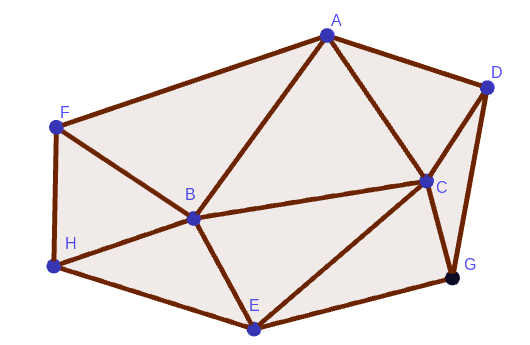
\includegraphics[scale=0.3]{Images/planar_graph}
\end{subfigure}%
\begin{subfigure}{.5\textwidth}
  \centering
  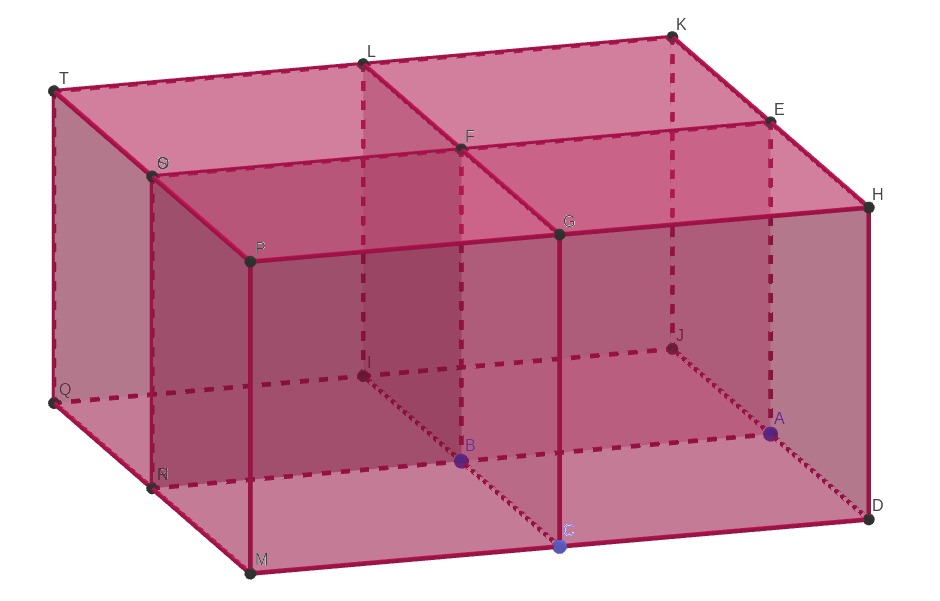
\includegraphics[scale=0.18]{Images/4cubes}
\end{subfigure}
\caption{\textbf{Gauche} : Graphe planaire ($|V|=8$,$|E|=15$,$|F|=9$). \textbf{Droite} : Polyèdre ($|V|=18$,$|E|=33$,$|F|=20$,$|T|=4$)}
\label{fig:planar_graph_4cubes}
\end{figure}
\noindent

\subsubsection{Cas surfacique}
\label{combi_2d}
\noindent
Dans le cas surfacique, la formule devient :
\begin{equation}
\label{eq:euler_surfacique}
\chi = |V|-|E|+|F|
\end{equation}
\begin{itemize}
\item $V$ est l'ensemble des sommets
\item $E$ est l'ensemble des arêtes
\item $F$ est l'ensemble des faces (ie. polygones)\\
\end{itemize}
Si nous sommes dans le cadre d'une triangulation surfacique et sans trou, alors chaque face est bordée par 3 arêtes et chaque arête n'étant par sur les bords appartient à 2 faces. Par conséquent $3F\leqslant 2E$. Ainsi l'équation \ref{eq:euler_surfacique} devient :\\
\begin{align*}
2 &\leqslant |V| - |E| + \frac{2}{3}|E| = |V| - \frac{1}{3}|E|\\
|E|&\leqslant 3|V|-6
\end{align*}
Il y a donc dans une triangulation surfacique environ 3 fois plus d'arêtes que de sommets.
\subsubsection{Cas volumique}
\noindent
Pour un maillage volumique, la formule d'Euler contient un terme de plus :\\
\begin{equation}
\chi = |V|-|E|+|F|-|T|
\end{equation}
\begin{itemize}
\item $T$ est l'ensemble des polyèdres (tétraèdres, hexaèdres...)\\
\end{itemize}
Si l'objet considéré est une variété alors chaque facette qui n'est pas sur les bords du volume est partagée par deux polyèdres, alors :\\
\begin{equation}
|F|\simeq 2|T|
\end{equation}
Ainsi :
\begin{equation}
\chi \simeq |V|-|E|+|T|
\end{equation}
Il y a donc autant d'arêtes que de polyèdres et sommets réunis (Tab. \ref{tab:caract_maillages}).

\subsection{Représentation des maillages tétraèdriques}
\label{representation_maillages_tetra}
\noindent
Ce rapport se concentre sur les structures de données pour maillages tétraèdriques. Comme rappelé dans l'introduction, une structure de données doit fournir une implémentation des opérateurs permettant la navigation et l'accès à la combinatoire du maillage (décrite par les relations d'incidence entre ses éléments). Dans le cas de maillages tétraèdriques, il est usuel de disposer des opérations suivantes:
\begin{itemize}
\item \texttt{incident\_face($i,t$)}: renvoie la $i$-ème face du tétraèdre $t$ (pour $i=0..3$).
\item \texttt{incident\_vertex($v$)}: renvoie un des tétraèdres incidents au sommet $v$.
\item \texttt{neighbour($i, t$)}: renvoie le tétraèdre qui est le $i$-ème voisin adjacent au tétraèdre $t$. 
\item \texttt{get\_vertex\_index($v,t$)}: renvoie un entier $i\in\{0 \ldots 3 \}$, l'indice du sommet $v$ dans le tétraèdre $t$.
%\indent \texttt{degree(i)} Cette fonction doit permettre de calculer le degré d'un sommet\\
%\indent \texttt{hypersphere(i)} Cette fonction doit retourner l'hypersphère ou l'étoile d'un sommet, c'est à dire l'ensemble des tétraèdres possédant le ième sommet.\\
%\indent \texttt{breadth\_first\_search(t)} Cette fonction doit permettre de réaliser un parcours en largeur du maillage en commen\c cant par le tétraèdre t .\\
\end{itemize}
\noindent
La combinaison de ces fonctions permet de réaliser la quasi-totalité des opérations de navigation locale qui sont effectuées habituellement
dans le cadre des procédures de modélisation géométrique et géométrie algorithmique. A titre d'exemple, on peut implémenter de manière efficace les fonctions suivantes:
\begin{itemize}
\item \texttt{degree($v$)}: renvoie le degré d'un sommet $v$
\item \texttt{hypersphere($v$)}: renvoie l'hypersphère ou l'étoile d'un sommet $v$, c'est-à-dire l'ensemble des tétraèdres incidents à $v$.
\item \texttt{BFS($t$)}: réalise un parcours en largeur du maillage en commen\c cant par le tétraèdre $t$.
\end{itemize}
On dit que la structure de données est \emph{indexable} si, de plus, elle permet l'accès en temps constant aux éléments du maillage (ses faces, sommets, ...), par le biais des opérations suivantes:
\begin{itemize}
\item \texttt{tetrahedron($i$)}: donne accès au $i$-ème tétraèdre,
\item \texttt{vertex($i$)}: donne accès au $i$-ème sommet.
\end{itemize}
Ces deux opérations sont parfois importantes dans plusieurs applications: elles permettent, par exemple, d'itérer sur tous les sommets ou tétraèdres,
ainsi que de récupérer les attributs qui y sont associés (couleurs, normales, coordonnées, ...).

\paragraph{Implantation naïve}
Une solution simple à implémenter (utilisée, entre autres, par la librairie \texttt{CGAL}~\cite{CGAL}) permettant de représenter un maillage tétraèdrique consiste à stocker explicitement les relations d'adjacence entre tétraèdres voisins et les relations d'incidence tétraèdre/sommet. Plus précisément, on stocke pour chaque tétraèdre plusieurs références : 
\begin{itemize}
\item $4$ références par tétraèdre donnant l'accès aux tétraèdres voisins
\item $4$ références par tétraèdre donnant l'accès aux sommets incidents
\item $1$ référence par sommet donnant l'accès à l'un de ses tétraèdres incidents
\end{itemize}
Au total, on comptabilise donc $8$ références par tétraèdre et $1$ référence par sommet ($8|T|+|V|$)~\footnote{Lorsqu'on parle de références il peut s'agir, selon le langage de programmation et environnement de travail choisi, de pointeurs (comme en \texttt{C/C++}), 
de références (comme en \texttt{Java}), ou d'indices si l'implémentation mise en place fait appel à des tableaux d'entiers (dans ce cas une référence vers un tétraèdre co\^utera
$\lceil\log_2 |T|\rceil$ bits).}.
\section{Etat de l'art}
\noindent
Les maillages sont la pluspart du temps stockés sous forme indexés. Dans un premiers temps, on énumère pour chaque sommet ses coordonnées géométriques. Puis pour chaque face (resp. tétraèdre), les indices de ses 3 (resp. 4) sommets. D'autres attributs peuvent être stockés (normales, couleurs...) mais nous n'en discuterons pas ici. Les formats indexés ne sont pas les formats les plus concis pour sauvegarder des maillages. En effet, la connectivité occupe une place très importante. Tandis que dans les maillages triangulaires surfaciques, le degré moyen d'un sommet est 6, il est de 22 dans les maillages tétraèdriques. Par conséquent, dans ce type de format, un sommet apparaitra dans 22 tétraèdres différents.\\
%La compression de maillages peut être séparer en 3 catégories : simplification polyhedrale, compression de positions, compression des informations de connectivités.\\\\
%\textbf{La simplification polyhedrale} consiste à simplifier le maillages en réduisant le nombre de sommets et en modifiant leurs positions afin que le nouveaux maillages reste aussi proche que possible de l'ancien. Ce sont des compression de maillages avec perte et ne sont donc pas adaptés aux usages nécessitant le maillage exact.\\\\
%\textbf{Compression des positions}\\\\
%\textbf{Compression de la connectivite}. La compression des informations de connectivité permet de réduire la redondance d'informations d'adjacence entre les k-simplexe d'un k-objet.\\\\
%En effet, comme dit dans la première partie, la structure de données doit être capable de répondre à des requetes simples (ex: donner les tetras adjacents à un tetra). Sans compression, cela signifie que chaque tetra doit stocker 4 références vers ses 4 tetras voisins. De plus, si l'on veut connaître les sommets composants un tetra, il est nécessaire de sauvegarder 4 references vers les 4 sommets composant le tetra. Ainsi, nous avons 8 références par tetra. Par conséquent, dans un maillage contenant 10000 tetras et en utilisant des références sur 32 bits, nous utiliserions 10000*8*32=2mo de références.
%On distingue les algorithmes de compression de maillages des structure de données pour maillages. Les premiers tentent de limiter au maximum l'usage mémoire du maillage en compressant le maillage. Le maillage devient inutilisable sous forme compressé, il est nécessaire de le décompresser pour l'utiliser à nouveau. En revanche, la structure de données pré-traite le maillage mais le maillage reste utilisable sous forme compressé.\\
La mesure utilisée pour évaluer la qualité d'une compression est le nombre de bits par sommets (bits per vertex ou bpv) tandis que la mesure utilisée pour évaluer la qualité d'une structure de données compacte est le nombre de références par triangle (resp. tétraèdre) rpt pour les maillages surfaciques (resp. volumiques).\\
On peut compresser un maillage en le simplifiant (supprimer des sommets...), en encodant la géométrie et/ou la connectivité du maillage. Nous ne nous intéresserons dans cette partie qu'à la compression de la connectivité puisque c'est la plus gourmande en mémoire. Par ailleurs, nous détaillerons d'abord le travail effectué dans le cadre surfacique puis volumique. Bien que notre travail soit uniquement centré sur les maillages volumiques, l'essentiel des travaux effectués jusqu'à présent est consacré aux maillages surfaciques.
\subsection{Maillages 2D}
\subsubsection{Compression}
\noindent
\textbf{Bande de triangle}. Les bandes de triangles ("triangles strips") et les eventails de triangles ("triangle fans") sont des représentations utilisées pour transférer les maillages de la mémoire centrale du PC vers la mémoire du GPU. Une bande de triangle est une séquence de sommet où chaque nouveau sommet défini un triangle avec les deux précedent sommets. En ce qui concerne les bande de triangles, le but est de trouver de très longues bandes. Si les bande de triangles sont suffisament longue alors, cette representation permet de passer de 3N references aux sommets à N+2. L'algorithme de Deering utilise ces bandes de triangles et utilise entre 3.3 et 9.8 bpv \cite{triangle_strips}.\\
\textbf{Traversée de triangles}. La Cut border Machine \cite{cut_border_machine_2d} est un algorithme de Gumhold qui encode la conectivité en parcourant le graphe en largeur. L'algorithme étend la frontière défini par un triangle initial en travesant itérativement des triangles adjacents. Sept symboles sont utilisés pour préciser si la frontière a été étendu en insérant un nouveau sommets, si la frontière a été séparée ou si deux frontière se sont jointes. Le schéma peut compresser des variétés avec 4 bpv. En revanche, ce résultat est seulement valide pour des maillages réguliers. En effet, quand une jointure est effectuée, un décallage doit etre fait pour désigner les sommets concernés. Par conséquent, il n'y a pas de borne supérieure garantie pour la compression avec cet algorithme.\\
L'algorithme EdgeBreaker de Rossignac \cite{edgebreaker} traverse lui aussi le graphe d'un triangle adjacent à un autre et enregistre la connectivité d'un maillage en produisant les sympboles C,L,R,E,S. Cependant, il garantit un cout de 4bpv.\\
\textbf{Codage de la Valence}. Une manière de décrire la connectivités de sommets est à travers leurs valence. Le premier travail sur la valence des sommets est le travail de Touma et Gotsman \cite{valence_encoding}. Le principe est de considérer la frontière d'un triangle initial et de l'étendre en ajoutant itérativement de nouveaux sommets. La connectivité est encodée en utilisant la valence des nouveaux sommets (concentrée autour de 6). Ainsi, La liste de valence des sommets peut être efficacement compressée par un encodeur d'entropie (2.3 bpv). C'est toujours aujourd'hui l'une des méthodes les plus efficace.
\subsubsection{Structure de données compacte}
\noindent
Plusieurs structures de données permettent une utilisation très facile des maillages et se focalisent sur l'utilisation des arêtes du graphe. C'est le cas d'Half-Edge, Winged-Edge \cite{winged_edge} et Quad-Edge qui stockent $19n$ références (soit 9.5 rpt). Elles permettent facilement de naviguer dans le maillage et opèrent des requêtes d'adjacence en temps constant. Cependant, elles occupent trop de place pour être considérées comme compactes.\\
La Corner Table (CT) est à la base de plusieurs structures de données. Elle utilise deux listes V et O de $3|F|$ entiers chacune où $F$ est l'ensemble des faces maillage. La table V stocke les incidences triangle/sommet tel-que les 3 sommets bordant un triangle t sont consécutifs (V[3t],V[3t+1],V[3t+2]) et sont listés dans un ordre consistent avec le maillage. Ainsi, V[c] représente un coin c associé avec une face f et un sommet. La table O stocke la référence entière du coin oposé. Le coin opposé o(c) au coin c est un coin dans un triangle adjacent qui partage la même arête opposée.\\
\begin{figure}[H]
\begin{center}
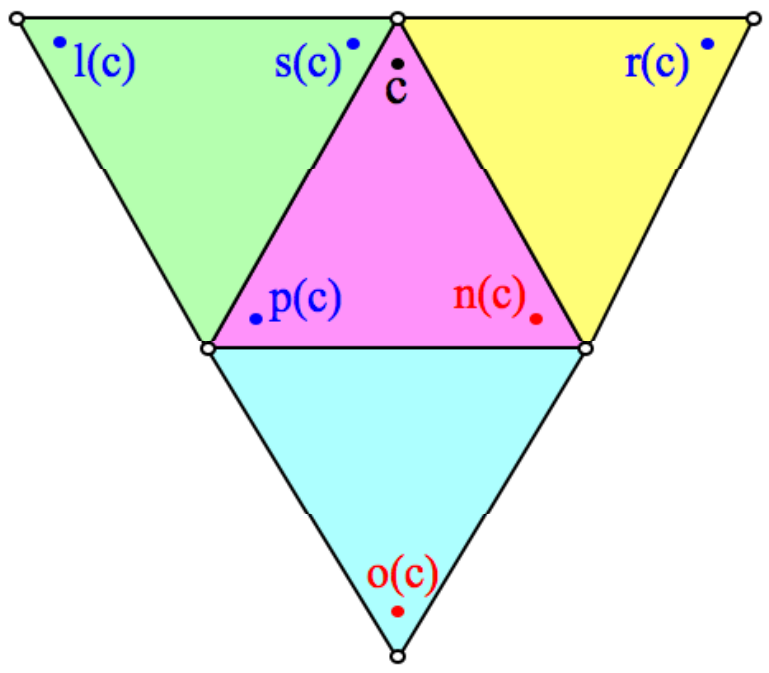
\includegraphics[scale=0.2]{Images/corner_table}
\caption{Les opérateurs utilisant les coins pour un maillage triangulaire}
\label{fig:corner_table}
\end{center}
\end{figure}
\noindent\ignorespacesafterend
\textbf{VOT}. La structure de données VOT (Vertex Opposite Table) est la première structure de données à utiliser cette 'Corner Table'. Elle permet une répresentation simple et efficace des maillages avec 6 références par triangle (3 références pour les sommets dans la table V et 3 références pour les coins dans la table O).\\
\textbf{SOT}. Développée par Rossignac \cite{SOT}, c'est une amélioration de VOT où la table O est réordonnée et la table V supprimée. Néanmoins, l'accès au coin d'un sommet et à l'étoile d'un sommet sont toujours en temps constant. Cette dernière structure de données utilise 3 rpt en moyenne.\\
\textbf{SQUAD}. Dans SQUAD \cite{squad}, les auteurs traversent le graphe en prodondeur afin d'appareiller les triangles deux à deux avec l'un de leurs sommet partagé. Cela leur permet d'avoir 4 références par quad (i.e pair de triangles) et donc d'économiser une référence par triangle. Quant aux triangles non appareillés, ils sont déguisés comme des quads. D'autre part, tout comme SOT, ils utilisent l'ordre des quads tel-que le ième quad soit associé au ième sommet. Dans un maillage surfacique, il y a deux fois plus de triangles que de sommets (cf. \ref{combi_2d}). Par conséquent, le nombre de quads et le nombres de sommets devrait être assez proche. Leur structure utilise en moyenne 2 rpt.\\
\begin{table}[th]
\footnotesize
\begin{tabular}{|c | c | c | c | c|}
\hline
Structure de données & Taille mémoire & Temps de navigation & Accès au sommet & Dynamique\\
\hline
Basées sur les arêtes & \multirow{2}{*}{18n+n} & \multirow{2}{*}{O(1)} & \multirow{2}{*}{O(1)} &\multirow{2}{*}{oui}\\
(Half-edge, Quad-edge, Winged-edge)&&&&\\
Basées sur les triangles & 13n & O(1) & O(1) & oui\\		
Corner table & 13n & O(1) & O(1) & oui\\
\hline
2D catalog \cite{2d_catalog}& 7.67n & O(1) & O(1) & oui\\
\hline
Star vertices \cite{star_vertices} & 7n & O(d) & O(1) & non\\		
SOT \cite{SOT}& 6n & O(1) & O(d) & non\\
SQUAD \cite{squad}& $(4+\epsilon)$n & O(1) & O(d) & non\\
%LR & $(2+\delta)$n & O(1) & O(d) & non\\
\hline  
\end{tabular}
\caption{Taille mémoire et performances des structures de données pour maillages surfaciques. n représente le nombe de sommets.}
\end{table}

\normalsize
%\subsubsection{Enumération de triangulations planaires}
%La connectivité d'un maillage peut etre vu comme un graphe. Pour les maillages surfaciques, les sommets sont des noeuds connectés via les arêtes du graphes pour former des faces.
%%Cette analogie entre maillage et graphe explique pourquoi certains résultats très connu de la théorie des graphes peuvent etre appliqués pour la compression de la connectivité des maillages.
%Tutte a d'abord proposé une formule pour énumérer les triangulations planaires. Cette première énumeration permet de calculer ce que l'on appelle l'entropie de Tutte. Cette entropie vaut environ 3.25 bpv (bits per vertex). C'est une borne supérieure pour l'entropie de la connectivité de n'importe quel maillage surfacique.
\subsection{Maillages 3D}
\subsubsection{Compression}
\noindent
\textbf{Grow\&Fold}. L'algorithme Grow\&Fold \cite{grow_and_fold} combine les idées de l'algorithme Topological Surgery \cite{topological_surgery} de Taubin et EdgeBreaker \cite{edgebreaker} de Rossignac. Il construit un arbre couvrant de tétraèdres et un folding string. L'arbre couvrant débute à une face arbitraire et grandit en ajoutant des tétraèdres aux faces externes de l'actuel arbre couvrant. Pour chaque ajout de tétraèdre, 3 bits encodent si d'autres tétraèdres seront attachés aux 3 faces extérieures de ce tétraèdre. Le folding string contient pour chaque triangle externe de l'arbre couvrant un code sur 2 bits permettant de retrouver les relations d'incidences absentes de l'arbre couvrant. L'arbre couvrant contient $|T|$ tétraèdres et il y a $2|T|$ faces externes. Par conséquent, l'usage mémoire est en moyenne de 7 bpt.\\
\textbf{Cut Border Machine}. La Cut Border Machine pour les maillages volumiques \cite{cut_border_machine_2d} est directement inspirée de celle pour les maillages surfaciques de Gumhold \cite{cut_border_machine_3d}. L'algorithme étend la frontière défini par une face initiale en traversant des tétraèdres adjacents. Dix symboles sont utilisés pour décrire l'entourage de la frontière lors de l'ajout d'un nouveau sommet pour la construction d'un tétraèdre. Leur algorithme permet de compresser les maillages tétraèdriques en utilisant 2.4 bpt et s'adapte aux non-variétés.
 
\subsubsection{Structure de données compacte}
\noindent
\textbf{VOT}. La Corner Table a été adapté par Rossignac aux maillages tétraèdriques (VOT). Elle demande 8 rpt (4 pour les sommets et 4 pour les coins opposés). Un index dans ces listes identifie un coin particulier à un tétraèdre. Ainsi, les tables O et V ont toutes les deux $4|T|$ entrées. Les coins de chaque tetrahèdre sont consécutifs dans les deux listes (les quatres coins du ième tetra sont stockées aux entrées  4i+j, where j = 0,1,2,3) et sont listés dans un ordre consistent avec l'orientation du tétrahèdre (les sommets des coins j=1,2,3 apparaissent dans le sens inverse des aiguilles d'une montre depuis le sommet du coin 0).\\
\textbf{Bande de Triangles}. Weiler et al. \cite{triangle_strips_weiler} encode les tétrahèdres en bandes. L'inclusion d'une petite quantité d'informations d'adjacence leur permet d'accéder aux faces voisines en temps constant. Leur algorithme stocke en moyenne 5.1 rpt.\\
\textbf{SOT}. La dernière structure de données développée est SOT \cite{SOT} par Rossignac. Elle améliore sa première structure de données VOT en triant la table O et en supprimant la table V. La structure de données utilise 4 références et 9 bits par tétraèdre en moyenne et permet l'accès à l'étoile d'un sommet en temps proportionel à son degré.

\begin{table}[th]
\footnotesize
\begin{tabular}{|c | c | c | c | c|}
\hline
Structure de données & Taille mémoire moyenne & Temps de navigation & Accès au sommet & Dynamique\\
\hline
VOT & 8t+n & O(1) & O(1) & oui \\
Bande de triangles \cite{triangle_strips_weiler} & 5.1t & O(1) & O(1) & non \\
SOT \cite{SOT} & 4t & O(1) & O(d)  & non\\
\textbf{Tétraèdre en diamants} & \textbf{ 2.4t } & \textbf{O(1)} & \textbf{O(d)} & \textbf{non} \\
\hline  
\end{tabular}
\caption{Taille mémoire et performances des structures de données pour maillages volumiques. t représente le nombre de tétraèdres et n le nombre de sommets}
\end{table}
\section{Notre Contribution : Tétraèdres en Diamants}
\subsection{Principe général}
\noindent
Notre algorithme s'inspire fortement de SQUAD. Seulement, appareiller les tétraèdres deux à deux permet seulement d'économiser une référence par cube, c'est à dire de passer de 4 références par tétraèdre à 3.\\
L'idée ici est de regrouper les tétraèdres partageant une même arête. On appelle un tel regroupement : \textbf{un diamant}. Notre algorithme plusieurs idées :
\begin{itemize}
\item Regroupement des tétraèdres comme SQUAD
\item Ancrer un sommet avec un diamant comme SOT
\item Ordonner les diamants tel-que le ième sommet soit au sein du ième diamant comme SOT
\item Passage d'un tétraèdre à l'autre en utilisant les faces (et non les coins)\\
\end{itemize}
Un diamant est un ensemble de tétraèdres adjacents deux à deux, partageant une arête commune et formant un cycle (Fig. \ref{fig:full_diamond2}). Dès lors que l'ensemble des tétraèdres n'est pas cyclique, la figure géométrique n'est plus un diamant (Fig. \ref{fig:not_full_diamond}).
\begin{figure}[H]
\centering
\begin{subfigure}{.5\textwidth}
  \centering
  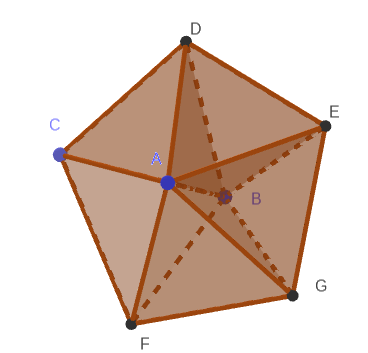
\includegraphics[scale=0.3]{Images/full_diamond}
  \caption{}
  \label{fig:full_diamond2}
\end{subfigure}%
\begin{subfigure}{.5\textwidth}
  \centering
  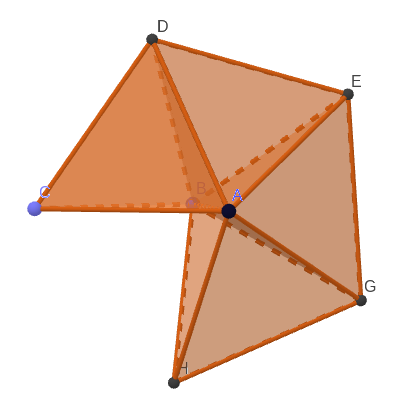
\includegraphics[scale=0.26]{Images/not_full_diamond}
  \caption{}
  \label{fig:not_full_diamond}
\end{subfigure}
\caption{\textbf{Gauche} : Exemple de diamant contenant 5 tétraèdres et dont l'arête centrale commune est AB. \textbf{Droite} : Exemple n'étant pas un diamant car les tétraèdres ne sont pas cycliques (bien que tous les tétraèdres partagent la même arête AB)}
%\label{fig:kvqkq}
\end{figure}
\noindent
Au sein d'un diamant, les tétraèdres sont ordonnés. Ainsi, on peut oublier les références de voisinage entre deux tétraèdres du même diamant. Pour les tétraèdres au sein d'un diamant, seules les références vers des tétraèdres extérieurs au diamant sont nécessaires. Un diamant $D_i$ contenant $|D_i|$ tétraèdres a $2|D_i|$ faces extérieures donc $2|D_i|$ références. Sur la Fig. \ref{fig:full_diamond2}, les faces ABD,ABE,ABG,ABF,ABC n'apparaitront pas dans notre structure car nous savons implicitement que pour passer d'un tétraèdre à l'autre dans ce diamant, nous utilisons une de ces faces.

\subsection{Appariement des tétraèdres en diamants}
\noindent
La première étape consiste à regrouper les tétraèdres en diamants. On peut ramener ce problème à un problème d'optimisation dans les graphes. En considérant notre maillage tétraèdrique comme un graphe (i.e en ne conservant que les arêtes et les sommets), il s'agit de choisir un ensemble $E'$ d'arêtes tel-que deux arêtes de $E'$ n'appartiennent pas au même tétraèdre. Les arêtes candidates pour appartenir à $E'$ sont toutes les arêtes qui ne sont pas situées sur les bords du maillage. Par exemple, sur Fig. \ref{fig:not_full_diamond}, l'arête AB est située sur le bord du maillage et n'est donc pas candidate pour appartenir à $E'$. Pour chaque arête selectionnée, le diamant est constitué de tous les tétraèdres possédant cette arête. Tous les tétraèdres n'ayant pas d'arêtes dans $E'$ sont appelés les tétraèdres isolés.\\
Pour trouver cet ensemble d'arêtes, nous avons essayé plusieurs algorithmes.
\subsubsection{Choisir une direction pour chaque sommet}
\noindent
La première méthode consiste à prendre pour chaque sommet, une arête dans une direction pré-définie. Néanmoins, cette méthode a deux inconvénients majeurs : deux arêtes peuvent être choisies et appartenir au même tétraèdre et elle utilise la géometrie du domaine (et donc peut sembler moins générique). Nous avons donc choisi de ne pas utiliser cette méthode.

\subsubsection{Optimisation aléatoire}
\noindent
Notre problème s'exprime facilement comme un problème d'optimisation combinatoire en nombres entiers. Malheureusement, la résolution de ces problèmes NP-difficile, ce qui signifie qu'aucun algorithme ne peut trouver une solution optimale en temps polynomial. Néanmoins, on peut utiliser des algorithmes d'optimisation aléatoire afin de trouver une solution approchée. Ce sont des algorithmes très utilisés en pratique qui visitent plus ou moins aléatoirement l'espace des solutions.\\
Soit $f$ la fonction aléatoire à maximiser, l'idée est de partir d'une solution initiale x et tant que la condition d'arrêt n'est pas remplie, de créer une solution y à partir de x puis de remplacer x par y si f(y)$>$f(x).\\
Dans notre cas, une solution est un ensemble d'arêtes. Elle est faisable si pour toute paire d'arêtes de notre solution, aucunes n'appartiennent au même tétraèdre. On peut donc matérialiser notre solution comme un vecteur de 0 et 1 pour chaque arête du graphe (1 si l'arête appartient à la solution, 0 sinon). Pour calculer la valeur de notre solution, on ajoute pour chaque arête de la solution le nombre de tétraèdres utilisant l'arête et si deux arêtes appartiennent au même tétraèdre alors on inflige une pénalité en soustrayant le nombre de tétraèdres adjacents à ces deux arêtes. L'inconvénient majeur de cet algorithme est sa lenteur. Il permet de trouver des solutions quasi optimales pour des maillages avec quelques milliers d'arêtes rapidement mais ne permet pas de trouver des solutions convenables au dela dans un temps raisonable. Nous avons donc décidé de ne pas retenir cette solution.

\subsubsection{Choisir l'arête de degré maximum}
\noindent
Le degré d'une arête est le nombre de tétraèdres possédant cette arête. Une heuristique très simple consiste à prendre en priorité les arêtes ayant un degré important. C'est un algorithme glouton dans la mesure où seulement la récompense immédiate nous intéresse. Il est nécessaire de trouver l'arête maximum à chaque itération de l'algorithme. Cela a pour conséquence un temps d'exécution relativement long.
\subsubsection{Parcours en largeur des tétraèdres}
\label{parcours_largeur}
\noindent
La troisième approche consiste à parcourir le maillage en largeur. On choisit un tétraèdre au début de l'algorithme puis on regarde pour chacune de ses arêtes si les tétraèdres partageant cette arète forment un diamant et qu'aucun n'appartienne déja à un diamant. Si ces deux conditions sont remplies, on crée un nouveau diamant avec cette arête centrale. Puis on ajoute à la file les tétraèdres adjacents et non visités au tétraèdre choisi. On exécute ainsi cet algorithme tant que la file n'est pas vide.\\
\begin{algorithm}[th]
\SetAlgoLined	
 Soit F une file;\\
 F.ajouter(t);\\
 \While{F n'est pas vide}{
  t = F.défiler();\\
  \For{arête e dans t}{
  \If{e forme un diamant}{
  \If{aucun des tétraèdres ayant e n'appartient à un diamant}{
  Creer un diamant avec e comme arête centrale;\\
  }
  }
  }
  Marquer t;\\
  Ajouter voisins de t non marqués à Q;
 }
 \caption{Parcours en largeur du maillage avec un tétraèdre de départ t}
\end{algorithm}

\begin{figure}[th]
\centering
\begin{subfigure}{.5\textwidth}
  \centering
  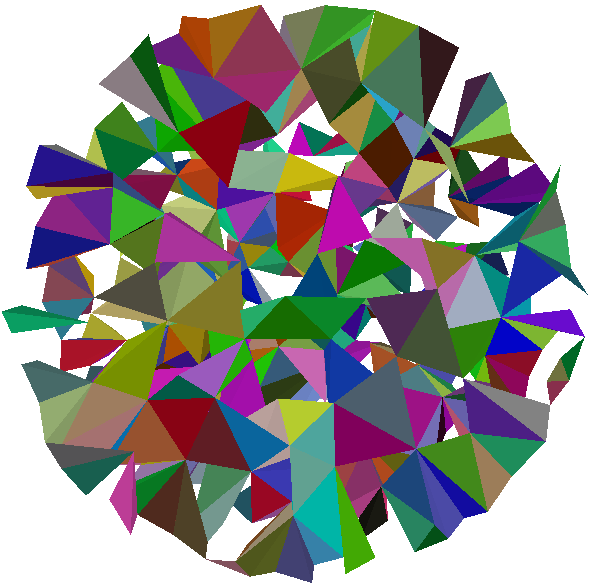
\includegraphics[scale=0.2]{Images/isolated_tetra}
  \caption{}
  \label{fig:isolated_tetra}
\end{subfigure}%
\begin{subfigure}{.5\textwidth}
  \centering
  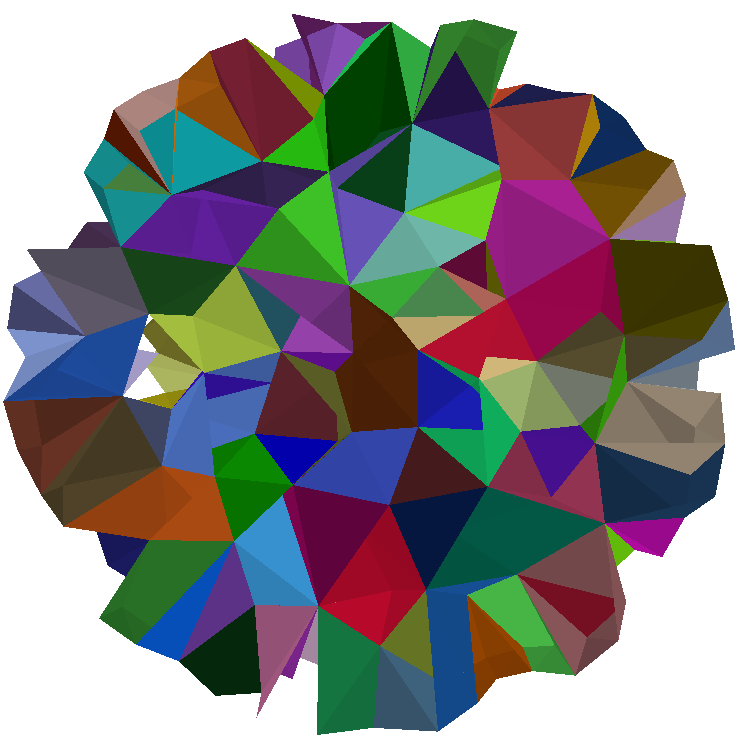
\includegraphics[scale=0.16]{Images/diamond}
   \caption{}
  \label{fig:diamond}
\end{subfigure}
\caption{\textbf{Gauche} : Vue de coupe des tétraèdres isolés après exécution du parcours en largeur pour créer les diamants. Chaque couleur représente un tétraèdre isolé. \textbf{Droite} : Vue de coupe des diamants après exécution du parcours en largeur pour créer les diamants. Chaque couleur représente un diamant.}
\end{figure}
\noindent
Sur Fig. \ref{fig:isolated_tetra}, on note une certaine homogénéité des tétraèdres isolés. En analysant plus spécifiquement la concentration des tétraèdres isolés, on remarque sur la Fig. \ref{fig:density_cow_hand} qu'ils sont particulièrement situé sur les bords et dans des régions à courbures \footnote{Afin que la densité ne soit pas biaisée, nous avons soustrait la densité originale du maillage. Le fait qu'une région soit plus densément peuplée en tétraèdres n'influence donc pas le résultat.}.
\begin{figure}[th]
\centering
\begin{subfigure}{.5\textwidth}
  \centering
  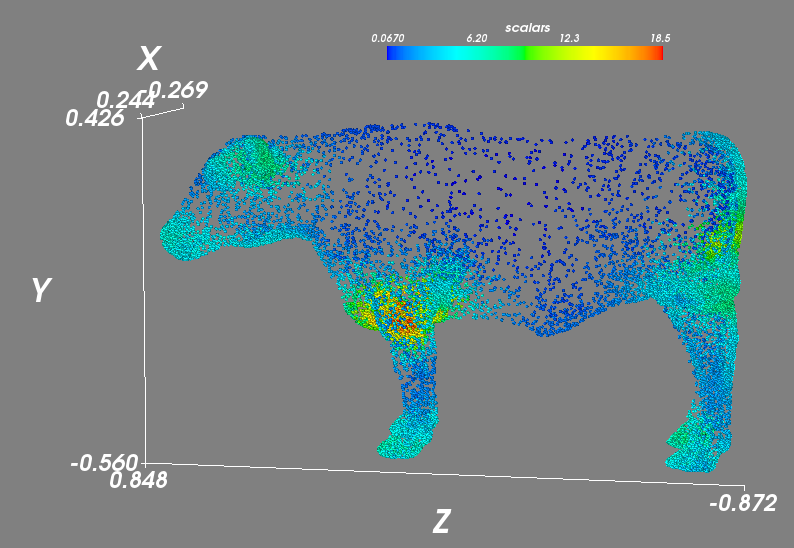
\includegraphics[scale=0.25]{Images/density_cow}
\end{subfigure}%
\begin{subfigure}{.5\textwidth}
  \centering
  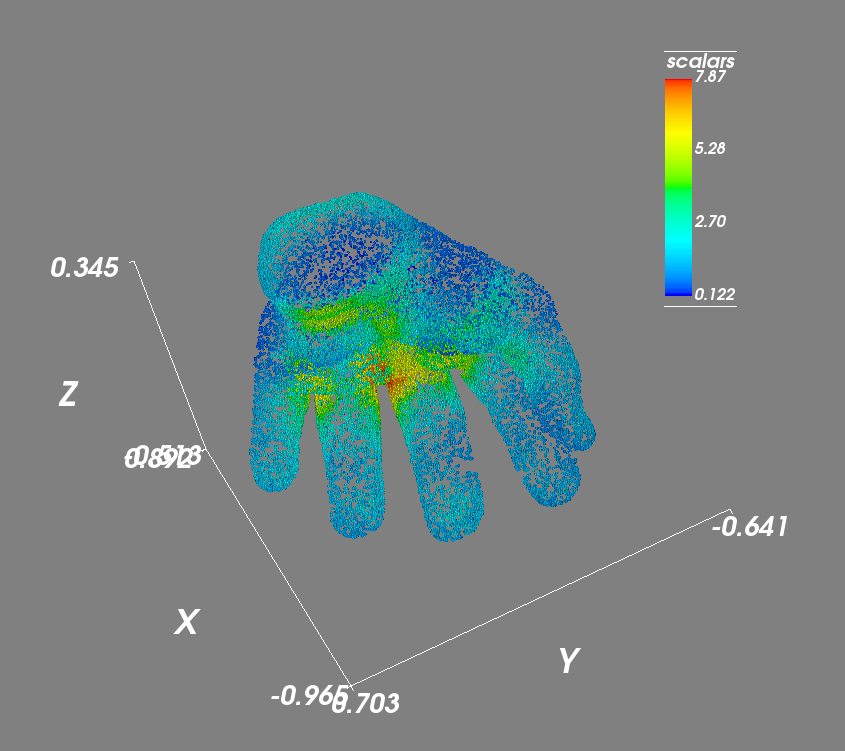
\includegraphics[scale=0.22]{Images/hand_density}
\end{subfigure}
\caption{Distribution des tétraèdres isolés. Chaque point représente le barycentre d'un tétraèdre et sa couleur indique la densité (le nombre de tétraèdres isolés à proximité).}
\label{fig:density_cow_hand}
\end{figure}

\paragraph{Choix du tétraèdre de départ}
Suivant le premier tétraèdre choisi pour lancer l'algorithme de parcours en largeur (Fig. \ref{fig:bfs_starting}), le taux de tétraèdres appareillés dans des diamants varie peu (1\% d'écart). Il semble néanmoins plus intéressant de commencer par les régions étroites.
\begin{figure}[th]
\begin{center}
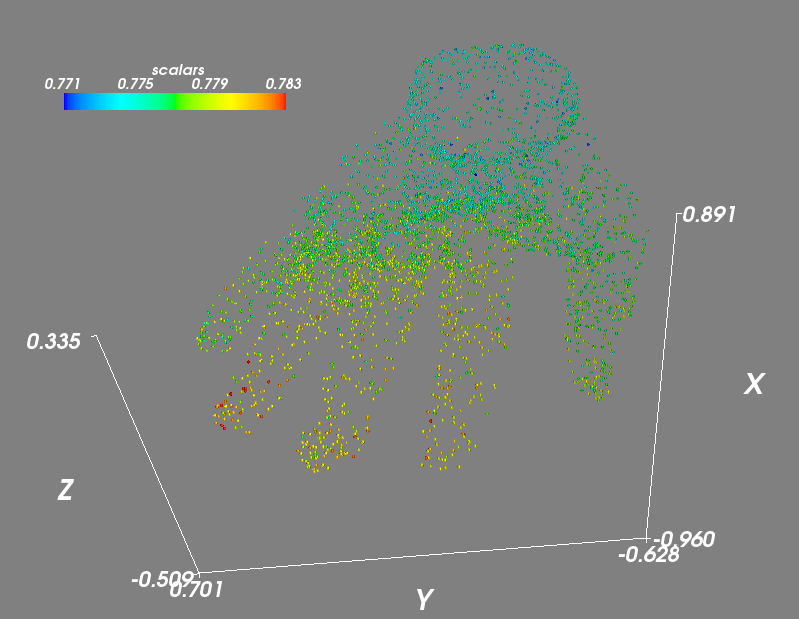
\includegraphics[scale=0.3]{Images/bfs_starting}
\caption{Performance de l'algorithme de parcours en largeur en fonction du tétraèdre de départ.}
\label{fig:bfs_starting}
\end{center}
\end{figure}

%\subsubsection{Résultats}


%\begin{tikzpicture}
%\begin{axis}[
%    title={Evolution des rpt en fonction du nombre de tétraèdres},
%    xlabel={Nombre de tétraèdres},
%    ylabel={RPT},
%    xmin=3000, xmax=2500000,
%    ymin=2, ymax=3,
%    xmode=log,
%%    xtick={0,20,40,60,80,100},
%%    ytick={0,20,40,60,80,100,120},
%    legend pos=north west,
%    ymajorgrids=true,
%    grid style=dashed,
%]
% 
%\addplot[
%    color=blue,
%    mark=square,
%    ]
%    coordinates {
%    (3583,2.69)(83412,2.39)(125127,2.44)(134707,2.44)(144037,2.37)(156135,2.44)(2243131,2.37)
%    };
%%    \legend{CuSO$_4\cdot$5H$_2$O}
% 
%\end{axis}
%\end{tikzpicture}

\subsection{Choisir l'ancre}
\label{ancrage}
\noindent
Le but de cette section est d'associer chaque sommet à un diamant ou un tétraèdre isolé. Voici les règles pour l'association.\\
\begin{itemize}
\item Un diamant ne peut être associé qu'à un sommet de son arête centrale
\item Un tétraèdre isolé peut être associé à n'importe lequel de ses quatres sommets
\item On associe en priorité les sommets à des diamants afin de calculer plus rapidement le degré du sommet\\
\end{itemize}
\begin{figure}[th]
\begin{center}
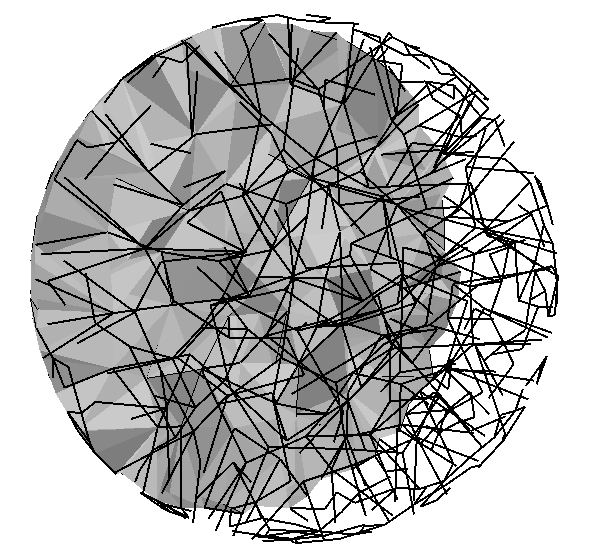
\includegraphics[scale=0.2]{Images/central_edges}
\caption{Vue de coupe d'une tétraèdrisation d'une boule avec affichage des arêtes centrales de tous les diamants}
\label{fig:central_edges}
\end{center}
\end{figure}
\noindent
Les différents cas possibles pour l'association des sommets sont les suivants :\\
\begin{itemize}
\item Le sommet est adjacent à une arête centrale disponible. On associe le sommet à cette arête.
\item Le sommet n'est adjacent à aucune arête centrale et il est adjacent à un tétraèdre isolé libre. Alors on associe le sommet à ce tétraèdre libre.
\item Le sommet n'est adjacent à aucune arête centrale, n'est pas adjacent à un tétraèdre isolé libre mais est adjacent à un diamant. On 'explose' alors le diamant, c'est à dire qu'on fait comme s'il était constitué que de tétraèdres isolés. Sur la Fig. \ref{fig:central_edge_AB}, le sommet F n'est pas sur une arête centrale. Si le diamant est déjà associé au sommet A (resp. B) alors on explose le diamant. On peut alors associer le sommet F (Fig. \ref{fig:explosion_diamond}) aux tétraèdres ABFG ou ABFC et le sommet A (resp. B) aux tétraèdres ACDB ou ADEB ou ABEG.\\
\end{itemize}

\begin{figure}[th]
\centering
\begin{subfigure}{.5\textwidth}
  \centering
  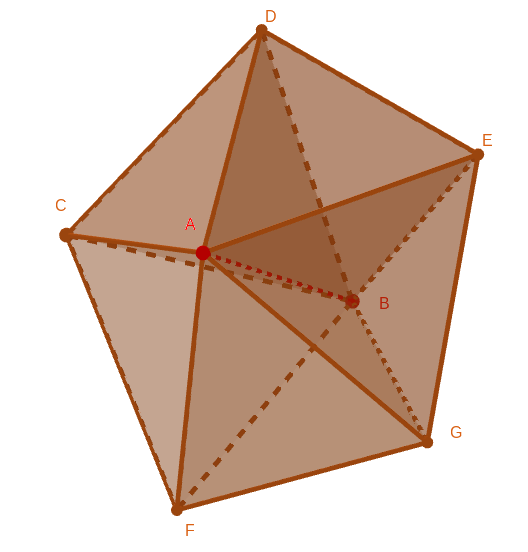
\includegraphics[scale=0.25]{Images/central_edge_AB}
  \caption{}
  \label{fig:central_edge_AB}
\end{subfigure}%
\begin{subfigure}{.5\textwidth}
  \centering
  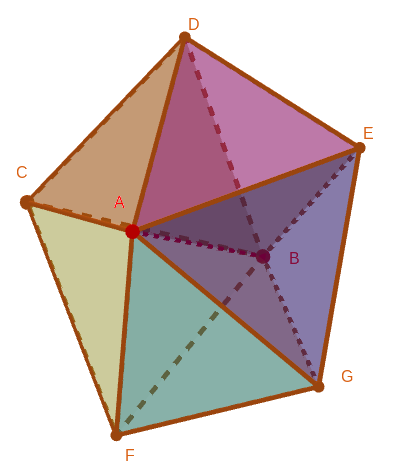
\includegraphics[scale=0.32]{Images/explosion_diamond}
  \caption{}
  \label{fig:explosion_diamond}
\end{subfigure}
\caption{\textbf{Gauche} : Diamant contenant 5 tétraèdres dont l'arête centrale est le segment AB et ancré au sommet A. \textbf{Droite} : 5 tétraèdres isolés (chaque couleur est un tétraèdre différent)}
\end{figure}
\noindent
Afin d'ancrer les sommets aux diamants/tétraèdres isolés, nous appliquons un algorithme glouton affectant en priorité les sommets adjacents à peu d'arêtes centrales et de tétraèdres isolés. Puis si nécessaire, nous explosons des diamants afin que tous les sommets soient appareillés avec des diamants/tétraèdres isolés différents.

\subsection{Organisation des diamant, tétraèdres et sommets}
\noindent
Les diamants sont construits et les sommets sont appareillés avec des diamants ou des tétraèdres isolés. Nous allons désormais apporter des précisions sur la manière dont sont ordonnés les diamants, tétraèdres et sommets.
\paragraph{Ordre des tétraèdres dans un diamant}
Au sein d'un diamant les tétraèdres sont ordonnés de manière purement arbitraire (Fig. \ref{fig:tetra_ordonnee}). La seule condition est que deux tétraèdres adjacents doivent avoir un ordre consécutif modulo le nombre de tétraèdres dans le diamant (ex: dans un diamant contenant 5 tétraèdres, le troisième tétraèdre doit être adjacent au deuxième tétraèdre et au quatrième).
\paragraph{Ordre des faces dans un diamant}
L'ordre des faces dans un diamant respecte celui des tétraèdres. Pour le ième tétraèdre dans un diamant, ses faces extérieures seront les faces $2i$ et $2i+1$. Si un diamant est associé à un sommet alors les faces paires sont adjacentes à l'ancre. Sur la Fig. \ref{fig:tetra_ordonnee}, l'ordre des face est donc : ACD,BCD,ADE,BDE,AGE,BGE,AFG,BFG,AFC,BFC.
\paragraph{Ordre des faces dans un tétraèdre isolé}
Les faces d'un tétraèdre isolé sont ordonnées de manière arbitraire. Seulement, si le tétraèdre isolé est ancré à un sommet, alors la première face doit être la face opposée à l'ancre.
\paragraph{Ordre des sommets dans les diamants}
\label{Ordre des sommets dans les diamants}Tout comme les tétraèdres, les sommets peuvent être ordonnés au sein d'un diamant. Un diamant $D_i$ possedant $|D_i|$ tétraèdres contient $|D_i|+2$ sommets. On ordonne d'abord les sommets situés entre deux faces (les sommets D,E,G,F,C sur la Fig. \ref{fig:tetra_ordonnee}), puis les deux sommets communs à toutes les faces (les sommets A et B sur la Fig. \ref{fig:tetra_ordonnee}). Le classement entre ces deux-derniers n'est pas important car on ne compare jamais l'ordre de ces deux sommets.\\
\begin{figure}[H]
\centering
\begin{subfigure}{.5\textwidth}
  \centering
  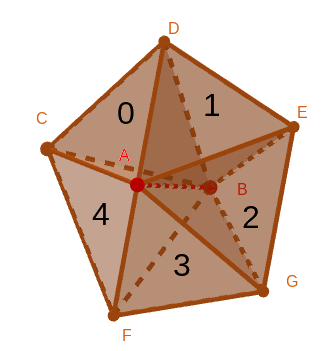
\includegraphics[scale=0.38]{Images/tetra_ordonnee}
  \caption{}
  \label{fig:tetra_ordonnee}
\end{subfigure}%
\begin{subfigure}{.5\textwidth}
  \centering
  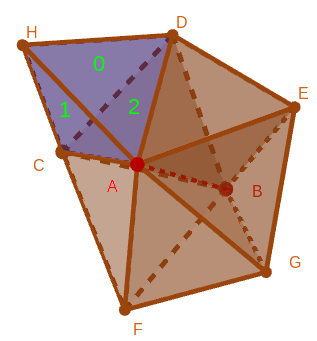
\includegraphics[scale=0.4]{Images/permutation_tetra_diamant}
  \caption{}
  
  \label{fig:permutation_tetra_diamant}
\end{subfigure}
\caption{\textbf{Gauche} : Diamant contenant 5 tétraèdres ordonnés, dont l'arête centrale est AB et ancré au sommet A. L'ordre des tétraèdres est indiqué en noir. L'ordre des sommets est : C,D,E,G,F,A,B. \textbf{Droite} : Un diamant partage une face avec un tétraèdre isolé. En vert est l'ordre des face du tétraèdre. L'ordre des sommets du tétraèdre est A,D,C,H et celui du diamant est C,D,E,G,F,A,B.}
\end{figure}
\noindent
%Calculer les permutations des sommets entre deux faces est primordial car cela permet de connaître la position d'un sommet dans la face opposée.\\
Avec la structure naïve décrite dans la partie \ref{representation_maillages_tetra}, chaque tétraèdre possède 4 références vers ses 4 sommets. Ainsi, pour deux tétraèdres adjacents, il suffit de comparer les références de leurs sommets respectifs pour identifier les sommets communs.\\
Ici, par soucis d'économie, nous ne souhaitons pas stocker de références des tétraèdres vers leurs sommets. Nous utilisons juste l'ordre des diamants et des tétraèdres isolés afin d'identifier la position d'un sommet (partie \ref{ancrage}).\\
Néanmoins, lorsque nous passons d'une face à l'autre, nous ne savons plus associer les sommets deux à deux. Dans la Fig. \ref{fig:permutation_tetra_diamant}, cela reviendrait à ne pas savoir lors du passage du tétraèdre isolé au diamant via la face ACD où se situe le sommet A (resp. C,D). Or, deux des opérations nécessaires à notre structure de donnée sont \textbf{degree(v)} et \textbf{hypersphere(v)} qui nécessitent toutes les deux d'identifier un sommet afin de parcourir les faces adjacentes à ce sommet. Par conséquent, pour connaître l'emplacement d'un sommet dans une face opposée, nous calculons des permutations.
Dans la Fig. \ref{fig:permutation_tetra_diamant}, pour calculer la permutation vue du tétraèdre isolé de la face CAD, il suffit de comparer l'ordre des sommets du tétraèdre isolé et du diamant. Si l'on garde seulement les 3 sommets qui nous intéressent dans les deux classements, on a : A,D,C et C,D,A. La permutation est donc (2,1,0). Bien entendu, la permutation pour la même face du point de vue du diamant est la même. Il y a 3!=6 permutations possibles et donc 3 bits par face sont nécessaires pour représenter ces permutations.

\subsection{La structure}
\noindent
Désormais, nos diamants sont formés, les sommets sont associés à des diamants (ou des tétraèdres isolés) et les permutations sont calculées pour chaque face du maillage. Nous introduisons quelques notations :
\begin{itemize}
\item $D$ l'ensemble des diamants
\item $T_D$ l'ensemble des tétraèdres appartenant à des diamants
\item $T_i$ l'ensemble des tétraèdres isolés
\item $F_e$ l'ensemble des faces des tétraèdres isolés et des faces extérieures des diamants où $|F_e|=2\cdot |T_D|+4\cdot |T_i|$\\
\end{itemize}
\noindent
La structure que nous proposons est un tableau A de taille $|F_e|$. Le tableau contient des entiers représentant les indices des faces. Ainsi A[i] indique l'indice dans le tableau de la face adjacente à la ième face. Si la ième face est sur le bord du volume alors A[i]=-1.\\ 
Un diamant contenant 4 tétraèdres occupera 8 cellules dans le tableau (car il a 8 faces extérieures) et un tétraèdre isolé en occupera 4. Les diamants et tétraèdres isolés sont ré-ordonnés de tel manière que le ième sommet soit ancré au ième diamant/tétraèdre isolé. Etant donné qu'il y a beaucoup plus de diamants que de sommets, seuls, les $|V|$ premiers diamants/tétraèdres isolés sont ré-ordonnés.\\
Par ailleurs, pour savoir quand on passe d'un diamant à un autre, nous utilisons des bits de service\footnote{Un bit de service est un bit permettant de faciliter une opération. Il prend si peu de place qu'on ne le considère par comme une référence (qui est souvent codée sur 32 bits)} (1 ou 0) pour chaque face. Une face contient un 1 si c'est la première face d'un diamant/tétraèdre isolé, 0 sinon. Finalement, afin de pouvoir tourner facilement autour d'un sommet, nous utilisons 3 bits de service par face pour représenter la permutation des sommets entre ces deux faces.\\
Pour résumer, voici notre structure de données :
\begin{itemize}
\item Un tableau A de taille $|F_e|$
\item Un bit de service par face afin de savoir si une face est la première d'un diamant ou d'un tétraèdre isolé
\item 3 bits de service par face afin de représenter la permutation des sommets entre deux faces
\end{itemize}
\begin{figure}[th]
\begin{center}
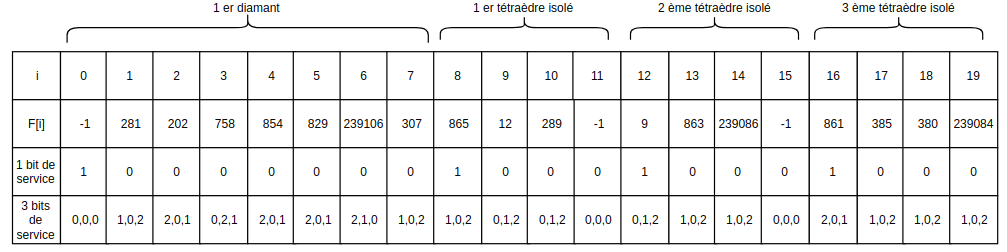
\includegraphics[scale=0.35]{Images/structure}
\caption{Notre structure est constituée d'un tableau A contenant les indices des faces adjacentes, d'un bit de service permettant de savoir si une face est la première d'un diamant ou d'un tétraèdre isolé, et de trois autres bits de service afin de connaître la permutation des sommets entre deux faces. Dans cet exemple, la face 0 est sur le bord et la face 1 est adjacente à la face 281. La permutation de la face 1 du premier diamant (1,0,2) indique que le premier et second sommets de cette face sont inversés dans la face opposée.}
\label{fig:structure}
\end{center}
\end{figure}

\paragraph{Ordre des sommets dans les tétraèdres}
Au sein d'un tétraèdre, les sommets sont ordonnés tel-que le ième sommet est opposé à la ième face. Si un sommet est associé au tétraèdre alors ce sommet est opposé à la première face.
\subsection{Les requêtes}
\noindent
Notre structure de données permet de réaliser des requêtes simples et courantes sur le maillage. Nous détaillons dans cette partie comment ces requêtes ont été implémentées et la complexité pour chacune d'elle.
\subsubsection{Accéder à la ième face}
\noindent
Pour accéder à la ième face, il suffit d'accéder à la cellule A[i] dans laquelle se trouve la face opposée à la ième face. L'accès est donc en temps O(1).
\subsubsection{Accéder au ième diamant ou tétraèdre isolé}
\noindent
Il suffit de parcourir le tableau A et de regarder pour chaque face si le premier bit de service vaut 1. On s'arrête alors dès que l'on a parcouru i faces dont la valeur du premier bit de service est 1. En utilisant une structure adaptée au 'Rank and Select' \footnote{Dans un tableau de bits $B[0..n-1]$, $rank(x) = |\{k\in [0..x] : B[k]=1\}|$ et $select(x)=min\{k\in [0..n-1) : rank(k)=x\}$}, la compléxité est O(1) \cite{rank_and_select}.
\subsubsection{Parcourir les tétraèdres d'un diamant}
\noindent
Les faces au sein d'un diamant sont ordonnées. Les faces consécutives dans le tableau (modulo la taille du diamant) sont adjacentes dans le diamant. Par conséquent, pour accéder aux faces du jème tétraèdre d'un diamant $D_i$, il suffit d'aller aux faces d'indices $2j$ et $2j+1$ (modulo $|D_i|$). La compléxité est O(1).
\subsubsection{Accéder au ième tétraèdre}
\noindent
Lors du regroupement des tétraèdres en diamants, l'ordre des diamants n'est plus le même que l'ordre initial (à la lecture du fichier OFF). Néanmoins, on peut re-ordonner les tétraèdres dans le fichier original afin que l'ordre des tétraèdres soit les mêmes. De cette manière on peut accéder au ième tétraèdre en O(1).
\subsubsection{Accéder au ième sommet}
\noindent
Bien que nous ne stockions pas les sommets de manière explicite (nous ne stockons que les faces). Nous sommes en mesures de localiser le ième sommet car il est adjacent au ième diamant/tétraèdre isolé.
Il suffit donc d'accéder au ième diamant/tétraèdre isolé. Si c'est un diamant, alors le sommet est adjacent à toutes les faces paires du diamant. Si c'est un tétraèdre isolé, alors le sommet est opposé à la première face et est donc adjacent au trois autres faces. La complexité est la même que pour accéder au ième diamant/tétraèdre isolé, O(1).
\subsubsection{Degré et hypersphère d'un sommet}
\noindent
Calculer le degré d'un sommet est plus compliqué. On sait que le ième sommet est adjacent au ième diamant/tétraèdre isolé. Si celui-ci est un diamant alors toutes les faces paires de celui-ci sont adjacentes au sommet ciblé. Si c'est un tétraèdre isolé, alors le sommet cible est opposé à la première face et est donc adjacent aux trois autres faces. Pour chaque face adjacente au sommet on accède à la face opposée en utilisant notre tableau A. En utilisant les permutations entre deux faces, nous sommes en mesure de savoir où se situe notre sommet dans la face opposée. Ainsi, nous pouvons accéder aux faces adjacentes au sommet dans ce nouveau diamant/tétraèdre isolé. Pour chaque diamant/tétraèdre isolé, on utilise un bit de service afin de savoir si celui-ci a déjà été visité \footnote{Nous omettons ce bit de service car il y en a en moyenne $\frac{|Diamants| + |T\acute{e}tra\grave{a}dres \; isol\acute{e}s|}{|T\acute{e}tra\grave{a}dres|}\simeq 0.5$ par tétraèdre}. On arrête de parcourir les faces quand tous les diamants et tétraèdres isolés adjacents au sommet ont été visités. La complexité est donc O(d).
\subsubsection{Parcours en largeur du graphe}
\noindent
Parcourir en largeur le graphe est plus facile que de calculer le degré d'un sommet. Il suffit d'utiliser une file et un bit de service pour chaque tétraèdre afin de savoir si celui-ci a été visité. Le passage d'un tétraèdre à l'autre est rendu très facile grace à notre tableau représentant les faces adjacentes. La complexité est donc la même que dans le maillage original : O($|$T$|$).
\subsubsection{Retrouver l'indice d'un sommet}
\label{Retrouver l'indice d'un sommet}
\noindent
Retrouver l'indice d'un sommet est une procédure courante. En effet lorsque on est sur une face, on peut vouloir connaître les indices des trois sommets qui la compose. Pour connaître l'indice d'un sommet, on calcule son hypersphère. Puis pour chaque diamant ou tétraèdre isolé dans l'hypersphère dont l'indice de la première face est inférieur à la limite\footnote{La limite est l'index à partir duquel les diamant et tétraèdres isolés ne sont plus associés à des sommets}, on calcule alors l'hypersphère du sommet ancré. Il suffit de comparer l'hypersphère de notre sommet cible avec les hypersphère des sommets ancrés et de renvoyer l'indice du sommet ayant la même hypersphère. Cette opération peut s'avérer néanmoins très couteuse. La compléxité pour calculer l'hypersphère d'un sommet est O(d). En utilisant notre algorithme pour appareiller les tétraèdres en diamants, les sommets sont en moyennes adjacents à 8 diamants/tétraèdres isolés. Seulement parmi ces 8 diamants/tétraèdres isolés, en moyenne 65\% \footnote{$\frac{|Diamants|+|T\acute{e}tra\grave{e}dres\; isol\acute{e}s|}{|V|}$} auront un indice inférieur à la limite. Par conséquent, retrouver l'indice d'un sommet nécessite de calculer en moyenne 6 (0.65*8+1) hypersphères.

%\begin{tikzpicture}
%\begin{axis}[
%    title={Evolution des rpt en fonction du nombre de tétraèdres},
%    xlabel={Nombre de tétraèdres},
%    ylabel={Secondes},
%    xmin=3000, xmax=2500000,
%    ymin=0, ymax=100,
%    xmode=log,
%%    xtick={0,20,40,60,80,100},
%%    ytick={0,20,40,60,80,100,120},
%    legend pos=north west,
%    ymajorgrids=true,
%    grid style=dashed,
%]
% 
%\addplot[
%    color=blue,
%    mark=square,
%    ]
%    coordinates {
%    (3583,0.06)(83412,21.34)(125127,50.6 )(156135,96.71)(2243131,33.29)
%    };
%%    \legend{CuSO$_4\cdot$5H$_2$O}
% 
%\end{axis}
%\end{tikzpicture}

%\begin{table}[H]
%\footnotesize
%\centering
%\begin{tabular}{|c | c | c |}
%\hline
%Type de & Taille du & Mémoire consomée \\
%structure & tableau de diamant & totale (bits) \\
%\hline
%B1 & 9670 & 48374 \\
%B2 & 199314 & 996594 \\
%B3 & & \\
%M1 & 308464  & 1542344 \\
%C1 & 385248 & 1926264\\
%\hline  
%\end{tabular}
%\label{Tab:results_memory}
%\caption{Tableau décrivant la place mémoire occupée par notre structure (les 3 tableaux)}
%\end{table}
%\noindent

\subsection{Un nouveau format de stockage}
\noindent
Les fichiers OFF encodent d'abord les coordonnées géométriques de chaque sommet puis les indices des 4 sommets de chaque tétraèdre. Ils sont ainsi très faciles à manipuler mais ne sont pas concis (un sommet apparaît en moyenne 22 fois dans une tétraèdrisation). L'idée de cette section est de tirer avantage de notre appariement des tétraèdres en diamants afin de sauvegarder les maillages dans un format plus succint.
\paragraph{Encodage de la structure}
Comme exprimé dans la partie \ref{Retrouver l'indice d'un sommet}, un sommet dans notre structure est adjacent en moyenne à 8 diamants/tétraèdres isolés. Par conséquent, plutôt que de décrire pour chaque tétraèdre les 4 indices des 4 sommets, nous pouvons encoder les indices des sommets composant un diamant. Les sommets sont ordonnés dans un diamant (\ref{Ordre des sommets dans les diamants}). Ainsi, en ayant juste l'ordre des sommets, nous sommes en mesure de retrouver les faces (la première face est bordée par le premier, le deuxième et l'avant dernier sommet).\\
Cependant, notre structure ne stocke pas implicitement les sommets. Nous savons seulement que le ième sommet est adjacent au ième diamant/tétraèdre isolé. Néanmoins, en calculant l'hypersphère d'un sommet, nous informons les faces adjacentes qu'elles possèdent ce sommet. En faisant ainsi pour tous les sommets du maillage, nous associons alors à chaque face ses 3 sommets bordants.\\
Il est alors facile de retrouver l'ordre des sommets dans un diamant à partir des sommets bordants chaque face du diamant. Il suffit de prendre tous les sommets qui apparaissent exactement deux fois dans toutes les faces (i.e les sommets qui n'appartiennent pas à l'arête centrale). Puis de les ordonner afin qu'ils décrivent un cycle.\\
Par exemple, sur la Fig. \ref{fig:tetra_ordonnee}, à partir du calcul de l'hypersphère de chaque sommet, nous saurions alors que :
\begin{itemize}
\item Les faces 0 et 1 contiennent les sommets C et D
\item Les faces 2 et 3 contiennent les sommets E et D
\item Les faces 4 et 5 contiennent les sommets G et E
\item Les faces 6 et 7 contiennent les sommets F et G
\item Les faces 8 et 9 contiennent les sommets C et F\\
\end{itemize}
Trouver l'ordre des sommets est alors aisé. On commence par trouver le sommet commun à la première et dernière face (i.e C), puis le sommet commun à la première et deuxième face (i.e D) et ainsi de suite pour finalement obtenir : C,D,E,G,F,A,B (les deux derniers sommets sont communs à toute les faces).

\paragraph{Ecriture dans un fichier}
L'écriture dans un fichier suit le même procédé que pour les fichiers OFF. Nous écrivons d'abord les coordonées géométriques de chaque sommet. Puis nous écrivons pour chaque diamant et tétraèdre isolé l'ordre de ses sommmets.

\paragraph{Ouverture du fichier}
L'ouverture est similaire à l'encodage du maillage. Pour chaque diamant, l'ordre des sommets nous permet de connaître les faces. Pour chaque tétraèdre isolé, l'ordre n'est pas important étant donné que tous les sommets d'un tétraèdre sont adjacents.

\paragraph{Résultats}
En théorie comme en pratique, notre structure nous permet de reduire en moyenne la taille du fichier OFF de 44\% ($\frac{8}{18}$).

\subsection{Implémentation}
\noindent
Tout le code est implémenté en C\texttt{++} natif, sans l'aide d'aucune bibliothèque extérieure. Le code source est compilé avec g\texttt{++} sous Elementary OS. Tous les algorithmes ont été exécutés sur une machine avec un processeur i5-5300U et 16Go de RAM. L'ensemble du code est open-source et disponible sur github : \url{https://github.com/beaupletga/3D-Mesh-Compression}.\\
Des classes représentent chaque forme géométrique (sommet, tétraèdre, diamant) permettant un code modulable et facilement exploitable. Nous utilisons cette représentation sous forme de classe pour la construction de notre structure mais elle est tout à fait absente dans son utilisation. \\
En ce qui concerne cette dernière, le tableau A est un tableau d'entiers codés sur 32 bits. Bien que nous aurions pu inclure les 4 bits de services dans les 32 bits de chaque entier, nous avons préféré utiliser deux tableaux annexes pour représenter ces bits de service. Le premier bit de service est stocké dans un tableau de booléens et les 3 autres bits de service sont stockés dans un tableau d'entiers. En codant les indices dans le tableau $F$ sur 28 bits et en utilisant les 4 derniers bits comme bits de service, nous pouvons encoder des maillages ayant jusqu'à $2^{28}=268$ millions de faces.
\section{Résultats}
\subsection{Procédure d'évaluation}
\noindent
Nous devons évaluer notre structure afin de comparer ses performances aux résultats pré-existants. Pour cela, nous avons choisi une dizaine de maillages avec des formes, des tailles, et des tétraèdrisations différentes (Fig. \ref{fig:exemples_maillages}). Les boules ont été générées avec CGAL \cite{CGAL} en utilisant le module de génération de sphères implicites. Les autres tétraèdrisations ont été pris le site "Aim@Shape". Nous ne présentons les résultats de nos algorithmes que sur 8 de ces maillages.
\begin{figure}[th]
\centering
\begin{subfigure}{.24\textwidth}
  \centering
  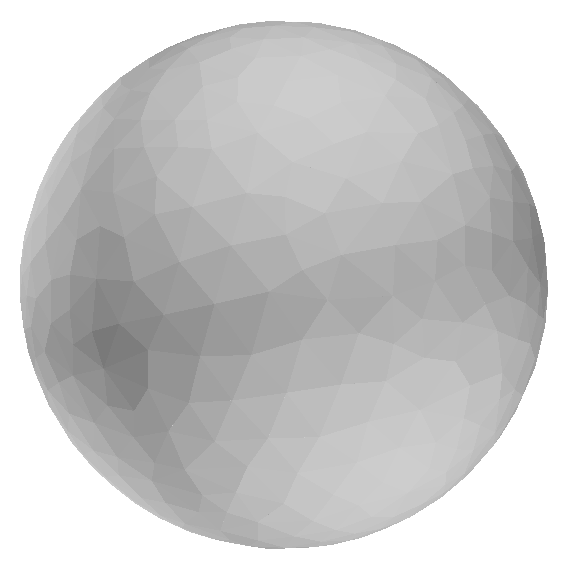
\includegraphics[scale=0.12]{Images/ball}
%  \caption{figure}{Tétraèdrisation d'une boule}
%  \label{fig:ball}
\end{subfigure}%
\begin{subfigure}{.24\textwidth}
  \centering
  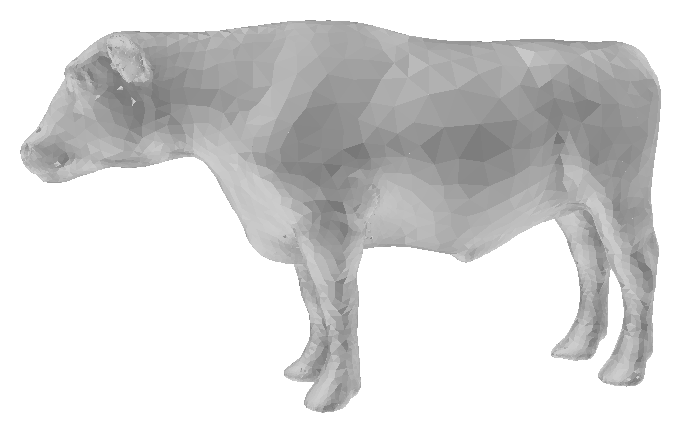
\includegraphics[scale=0.12]{Images/cow}
%  \caption{figure}{Tétraèdrisation d'une vache}
%  \label{fig:cow}
\end{subfigure}
\begin{subfigure}{.24\textwidth}
  \centering
  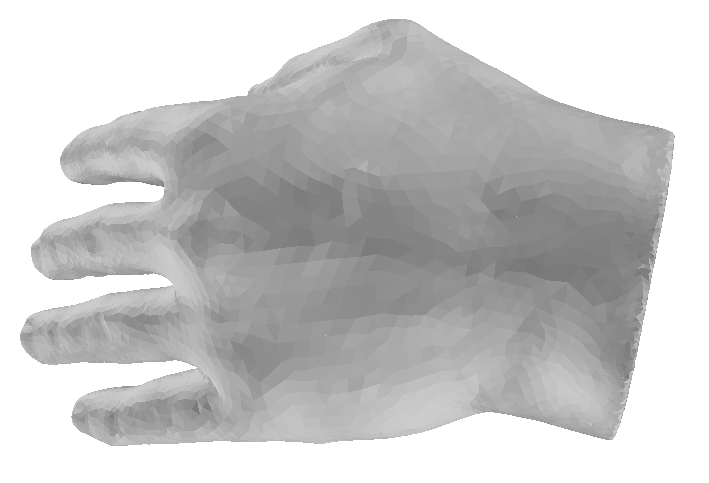
\includegraphics[scale=0.12]{Images/hand}
%  \caption{figure}{Tétraèdrisation d'une main}
%  \label{fig:hand}
\end{subfigure}%
\begin{subfigure}{.24\textwidth}
  \centering
  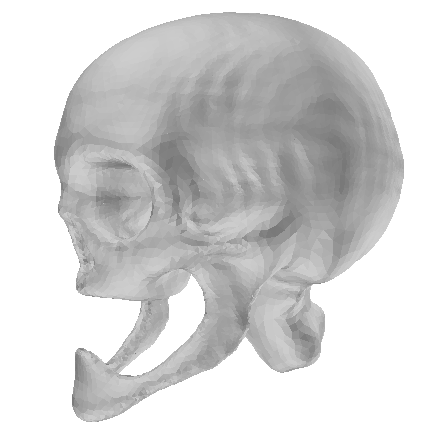
\includegraphics[scale=0.14]{Images/skull}
%  \caption{figure}{Tétraèdrisation d'un crane}
%  \label{fig:skull}
\end{subfigure}
\caption{Exemples de maillages tétraèdriques utilisés pour évaluer notre structure de données.}
\label{fig:exemples_maillages}
\end{figure}

\begin{table}[H]
\footnotesize
\begin{tabular}{|c | c | c | c | c| c | c |}
\hline
Nom de la & Nombre de & Nombre& Nombre de & Part de tétraèdres & Nombre de & Nombre d'arêtes\\
structure&sommets&d'arêtes &tétraèdres&sur les bords&tétraèdres par sommet & par sommet\\
\hline
Boule (B1) & 1k & 5k & 3k & 0.45 & 13.52 & 10.32 \\
Boule (B2)& 15k & 101k & 83k & 0.07 & 22.15 & 13.45\\
Boule (B3)& 378k & 2M & 2.2M & 0.05 & 23.70 & 13.98 \\
Boule (B4)& 1.3M & 9.5M & 8.1M & 0.01 & 24 & 14 \\
Boule (B5)& 1.7M & 12.1M & 10.3 & 0.01  & 24.03  & 14.01  \\
Vache (V1)& 30k & 182k & 134k & 0.24 & 17.48 & 11.82 \\
Main (M1)& 28k & 169k & 125k & 0.24 & 17.38 & 11.74\\
Crane (C1)& 37k & 217k & 156k & 0.30 & 16.51 & 11.52 \\ 
\hline  
\end{tabular}
\caption{Caractéristiques des maillages tétraèdriques utilisés pour évaluer notre structure}
\label{tab:caract_maillages}
\end{table}

\subsection{Appareillage en diamants}
\noindent
On peut évaluer l'appareillage des tétraèdres en diamants en regardant la part des tétraèdres dans des diamants ou en calculant le nombre de références par tétraèdre (rpt). On calcule ce dernier de cette manière :\\
\begin{equation}
\text{rpt} = \frac{2\cdot T_D+4\cdot T_i}{|T|}
\end{equation}
\begin{table}[H]
\centering
\footnotesize
\begin{tabular}{|c | c | c | c| c | c | c |}
\hline
& \multicolumn{3}{|c|}{Parcours en largeur}& \multicolumn{3}{|c|}{Degré de l'arête}\\
\hline
Nom de la & Part des tétraèdres & RPT & Temps (s) & Part des tétraèdres & RPT & Temps (s)\\
structure&dans des diamants (\%)&&&dans des diamants (\%)&&\\
\hline
B1 & 76 & 2.69 & 0.03 & 81 & 2.36 & 0.47 \\
B2 &  80 & 2.39 & 1.02 & 85 & 2.29 & 497 \\
B3 & 81& 2.37 & 39.79 &  &  &\\
B4 & 82& 2.35 & 150 &  &  &\\
B5 & 82 & 2.35 & 172 &  &  &\\
V1 & 77& 2.44 & 1.56 & 81& 2.36 & 922\\
M1 & 77& 2.44 & 1.26 & 83 & 2.34 & 794\\
C1 & 77& 2.44 & 1.48 & 80 & 2.38 & 1262\\
\hline  
\end{tabular}
\caption{Résultats des algorithmes d'appareillage des tétraèdres en diamants. Le deuxième algorithme ayant des temps de calculs assez importants, certains maillages n'ont pas pu être considérés.}
\label{tab:results_performances}
\end{table}

\begin{figure}[H]
\begin{center}
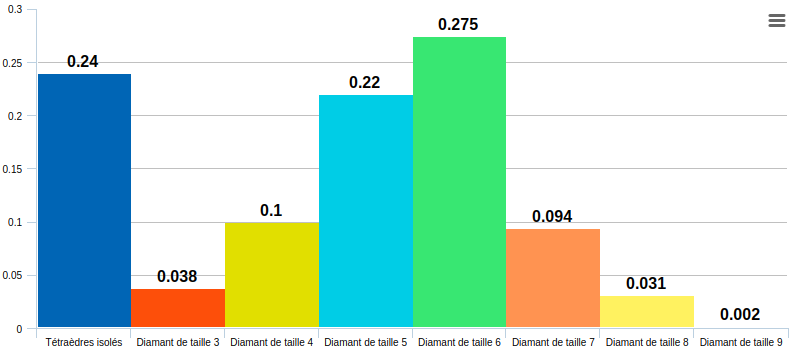
\includegraphics[scale=0.35]{Images/histograme}
\caption{Histogramme de la part de tétraèdres parmi les tétraèdres isolés et diamants en utilisant le parcours en largeur}
\label{fig:histogramme}
\end{center}
\end{figure}
\begin{figure}[H]
\centering
\pgfplotsset{width=15cm,height=5.5cm}
\begin{tikzpicture}
\begin{axis}[
    ybar,
    enlargelimits=0.15,
    legend style={at={(0.6,0.9)},
      anchor=north,legend columns=-1},
    ylabel={RPT},
    xlabel={Nombre de tétraèdres par arête},
    symbolic x coords={3.9,4.29,4.43,4.93,5.08,5.10,5.11},
    xtick=data,
    nodes near coords,
    nodes near coords align={vertical},
    ]
\addplot coordinates {(3.9,2.69)(4.29,2.44)(4.43,2.44)(4.93,2.39)(5.08,2.37)(5.10,2.35)(5.11,2.35) };
\addplot coordinates {(3.9,2.36)(4.29,2.38)(4.43,2.34)(4.93,2.29)(5.08,)(5.10,)(5.11,) };
\legend{Parcours en largeur,Arête de maximum degré}
\end{axis}
\end{tikzpicture}
\caption{Nombre de références par tétraèdre (rpt) en fonction du nombre de tétraèdres par arête}
\label{fig:graphique}
\end{figure}

\vspace{0.1cm}
\noindent
On note sur la Fig. \ref{fig:graphique} qu'il semble avoir un lien entre le nombre de tétraèdres par arête et les performances de nos algorithmes de création de diamants. Ce comportement ne semble pas étonnant étant donné que plus le nombre de tétraèdres par arête est important, plus les diamants peuvent contenir un nombre important de tétraèdres. Compte tenu des résultats de Tab. \ref{tab:results_performances}, nous avons choisi d'utiliser le parcours en largeur pour appareiller les tétraèdres en diamants. Le parcours en largeur est rapide et permet d'associer en moyenne 76\% des tétraèdres en diamants. Néanmoins, notre algorithme pourrait probablement être amélioré en étant exécuté en parallèle ou en choisissant plus spécifiquement un tétraèdre de départ (Fig. \ref{fig:bfs_starting}). On remarque que 50\% des tétraèdres sont dans des diamants possédant 5 ou 6 tétraèdres (Fig. \ref{fig:histogramme}).

\subsection{Ancrage des sommets}
\begin{table}[H]
\footnotesize
\centering
\begin{tabular}{|c | c | c | c |}
\hline
Nom de la & Part de sommets non associés & Part de tétraèdres dans  & Part de tétraèdres dans \\
structure&avec des diamants  & des diamants avant & des diamants après \\
& ou tétraèdres isolés (\%) & choix des ancres (\%)& choix des ancres (\%)\\
\hline
B1 & 6 & 76& 65 \\
B2 & 0.08& 80 & 80 \\
B3 & 0.03& 82 & 82\\
B4 & 0.01 & 82 & 82\\
B5 & 0.02 & 82 & 82\\
V1 & 0.8  & 77 & 76 \\
M1 & 0.7 & 77& 76\\
C1 & 0.8 & 77 & 76 \\
\hline  
\end{tabular}
\caption{Résultats de l'ancrage des sommets aux diamant/tétraèdres isolés en utlisant un algorithme glouton affectant en priorité les sommets adjacents à peu de diamants/tétraèdres isolés}
\label{tab:results_ancres}
\end{table}
\noindent
On remarque sur le Tab. \ref{tab:results_ancres} qu'en appliquant l'algorithme glouton afin d'appareiller sommet et diamant/tétraèdre isolé, une part minime des sommets demeure non ancrée (1ère colonne). Par ailleurs, on note que la destruction de certains diamants pour associer des sommets à des tétraèdres n'a que peu d'incidence sur la part de sommets ancrés tant que le nombre de sommets est important (2ème et 3ème colonnes).

\subsection{Les requêtes}
\noindent
Pour évaluer le temps nécessaire pour répondre à une requête, nous évaluons celle-ci après 10 000 essais aléatoires. Les temps sont obtenus en utilisant l'optimisation '-O3' de C\texttt{++}.
\begin{table}[h]
\footnotesize
\centering
\begin{tabular}{| c | c | c| c |c |c|}
\hline
Nom de la & Accès au& Accès au & Degré d'un & Parcours en & Parcours en\\
structure &ième tétraèdre (s)& ième diamant (s) &sommet (s)&largeur (s) & largeur normalisé\footnote{Par rapport au nombre de tétraèdres} (s/tétraèdre)\\
\hline
B1  & 1e-5 & 5e-6 & 1.9e-5 & 6e-4& 1.67e-7 \\
B2  &  4.1e-4 & 1.6e-4 & 1.2e-4 & 0.01& 1.19e-7\\
B3 & 0.011 & 0.0042 & 0.002 & 0.8&3.56e-7\\
B4 & 0.01 & 0.01 & 0.01 & 4.6&5.6e-7\\
B5 & 0.04 & 0.01 & 0.01 & 4.46& 4.3e-7 \\
%V1 & & & & \\
M1  & 6.4e-4 & 2.6e-4 & 2.2e-4 & 0.02&1.59e-7\\
C1  & 8.1e-4 & 3.4e-4 & 2.8e-4 & 0.02&1.28e-7\\
\hline  
\end{tabular}
\label{table:results_time}
\caption{Temps requis (s) pour répondre aux requêtes sur plusieurs maillages}
\end{table}
\noindent

%Temps moyen structure de données non compacte (4 references tétra)
%1.8e-3 7.8e-4 1.9e-4 0.36
%2.5e-3 9.9e-4 5.2e-4 0.17
%
\begin{figure}[H]
\centering
\pgfplotsset{width=12cm,height=7cm}
\begin{tikzpicture}
\begin{axis}[
    ybar,
    enlargelimits=0.1,
%    legend style={anchor=east},
    legend style={at={(0.62,0.94)}},
%    anchor=north,legend columns=-1,cells={align=left}},
    ylabel={Secondes (s)},
%    xlabel={Nombre de tétraèdres par arête},
    symbolic x coords={Accès au ième tétraèdre,Degré d'un sommet,Parcours en Largeur},
    xtick=data,
    nodes near coords,
    nodes near coords align={vertical},
    ]
\addplot coordinates {(Accès au ième tétraèdre,2.5e-3)(Degré d'un sommet,5.2e-4)(Parcours en Largeur,1.85e-3)};
\addplot coordinates {(Accès au ième tétraèdre,1.8e-3)(Degré d'un sommet,1.9e-4)(Parcours en Largeur,4.25e-3)};
%\addplot coordinates {(Degré d'un sommet,1e-3)(Parcours en Largeur,2.92e-3)};
%\addplot coordinates {(3.9,2.36)(4.29,2.38)(4.43,2.34)(4.93,2.29)(5.08,)(5.10,)(5.11,) };
\legend{Structure Compacte,Structure Compacte avec 4 rpt,Structure avec Pointeurs}
\end{axis}
\end{tikzpicture}
\caption{Comparaison des temps moyens (s) requis pour répondre aux requêtes avec notre structure de données compacte et une structure de données compacte utilisant 4 rpt (i.e SOT). Le temps pour le parcours en largeur est normalisé pour 100 000 tétraèdres.}
\label{fig:temps_moyen}
\end{figure}
\noindent
Sur Fig. \ref{fig:temps_moyen}, on constate que les temps de calcul de notre structure de données compacte sont moins bons pour l'accès au ième tétraèdre et le calcul du degré d'un sommet\footnote{Nous n'affichons pas le temps d'accès au ième diamant car la structure de données compacte à 4 rpt ne réunis pas les tétraèdres en diamants}. Etant donné que dans notre structure de données, le ième tétraèdre est plus proche du début du tableau que dans la structure à 4 rpt, le résultat devrait être l'inverse. De la même manière, pour le calcul du degré d'un sommet, sachant que les tétraèdres sont regroupés en diamants dans notre structure, le degré devrait être plus rapidement calculé. Nous expliquons ces deux écarts par les comparaisons effectuées dans les requêtes. En effet, lorsque nous voulons calculer le degré d'un sommet, si le sommet est adjacent à un tétraèdre isolé, alors il suffit de localiser la face du tétraèdre isolé non adjacente au sommet puis de naviguer au sein des trois autres faces. En revanche, lorsque notre sommet est adjacent à un diamant, davantage de comparaisons sont nécessaires afin de connaître les faces adjacentes au sommet. Cette suposition est confirmée en analysant les temps requis pour le parcours en largeur du graphe. Lorsque nous effectuons un parcours en largeur du graphe, aucune comparaison (utilisant les permutations des sommets) n'est nécessaire, il suffit seulement d'accèder au diamant/tétraèdres adjacents. Sachant que les tétraèdres sont regroupés en diamants dans notre structure, en accèdant à un diamant $D_i$, on accède directement au $|D_i|$ tétraèdres le composant, gagant un temps non négligeable. 
%Par ailleurs, nous avons choisi de d'ajouter à la comparaison une structure compacte (avec un regroupement en diamants) utilisant les pointeurs (et non un tableau d'entiers). On s'aper\c oit
\subsection{Taille mémoire}
\begin{figure}[H]
\centering
\pgfplotsset{width=13cm,height=7cm}
\begin{tikzpicture}
\begin{axis}[
    ybar,
%    ymode = log,
    enlargelimits=0.15,
    legend style={at={(0.4,0.94)},
      anchor=north,legend columns=-1,font=\fontsize{9}{9}\selectfont},
    ylabel={Mega Bytes (MB)},
    xlabel={Nombre de tétraèdres},
    symbolic x coords={2.2M,5.3M,8.1M,10.3M},
    xtick=data,
    nodes near coords,
    nodes near coords align={vertical},
    ]
%\addplot coordinates {(3k,9234)(83k,199262)(125k,307500)(156k,384156)(2.2M,5291508)(8.1M,19212158)(10.3M,24407986)};
%\addplot coordinates {(3k,14332)(83k,333648)(125k,500508)(156k,624540)(2.2M,8.97e6)(8.1M,3.26e7)(10.3M,4.14e7)};
\addplot coordinates {(2.2M,20.8)(5.3M,50.4)(8.1M,76.8)(10.3M,97.6)};
\addplot coordinates {(2.2M,35.6)(5.3M,85.6)(8.1M,130.4)(10.3M,165.6)};
\legend{Structure Compacte,Structure non Compacte (4 rpt)}
\end{axis}
\end{tikzpicture}
\caption{Comparaison de la taille mémoire (en bytes) de notre structure de données compacte et de la même structure de données sans regroupement des tétraèdres en diamants}
\label{fig:taille_memoire}
\end{figure}
\noindent
La Fig. \ref{fig:taille_memoire} compare l'évolution de la place mémoire en fonction du nombre de tétraèdres par maillages pour notre structure de données et une structure de données utilisant 4 références par tétraèdres. Cette dernière structure de données est équivalente à SOT, seulement elle utilise les faces plutôt que les coins pour naviguer dans le maillage. Sur le plus gros maillage, notre structure de données permet d'économiser 68MB de place mémoire.

%
%temps pour la structure non compacte
%B1 1.31e-5 5.3e-6 2.7e-5 9.1e-4
%B2 2e-4 & 1e-4 7.1e-5 0.03
%B3 8.1e-3 3e-3 7e-4 1.8
%B4 
%M1 4.9e-4 1.9e-4 8.6e-5 0.04
%C1 6.4e-4 2.7e-4 1.1e-4 0.06


\section{Partie Théorique}
\subsection{Borne inférieure théorique}
\subsection{NP-Complétude}
\noindent
La pierre angulaire de notre structure est la constuction des diamants. Si tous les tétraèdres étaient regroupés en diamants, alors nous achèverions un encodage de la connectivité avec 2 rpt. Le parcours en largeur est satisfaisant mais existe-il un algorithme optimal en temps polynomial ? Nous allons montrer dans cette section que le problème est en réalité NP-dur.\\
Notre problème est le suivant : \textbf{Existe-il une couverture des tétraèdres en diamants contenant plus de k diamants ?}\\
Pour cela, nous allons procéder en 4 étapes :
\begin{enumerate}
\item Montrer que notre problème est NP
\item Transformer notre maillage tétraèdrique en graphe en temps polynomial
\item Résoudre MIS sur ce nouveau graphe
\item Montrer que si l'on a une solution de MIS sur ce graphe alors on a une solution pour notre problème.
\end{enumerate}
Pour rappel, notre problème consiste à choisir un ensemble $E'$ d'arêtes tel-que deux arêtes de $E'$ n'appartiennent pas au même tétraèdre.\\
1- Commencons par montrer que notre problème appartient à NP. Une solution est un ensemble d'arêtes (les arêtes centrales des diamants). Il suffit de vérifier pour chaque arête que A COMPLETER
2- On peut créer un autre graphe où chaque arête du graphe initial est modélisée par un sommet. Deux sommets dans ce nouveau graphe sont connectées si et seulement si leurs arêtes dans le graphe original appartiennent au même tétraèdre. La création de ce nouveau graphe se fait en temps polynomial (en fonction des arêtes).\\
3- Calculer un Stable Maximum (Maximum Indepent Set ou MIS en anglais) sur ce nouveau graphe signifie trouver un ensemble de sommets non connectés dans le graphe. C'est équivalent à trouver un ensemble d'arêtes n'appartenant pas aux mêmes tétraèdres dans notre maillage.\\
4- Ainsi, calculer un MIS sur ce nouveau graphe est similaire à trouver un ensemble d'arêtes (et donc de diamants) indépendants.\\
5- Par conséquent, trouver une solution à notre problème signifierait trouver une solution au MIS\\
Nous avons donc réduit notre problème au MIS. Notre problème est donc NP-Dur.
\section{Travail Futur}
\subsection{Améliorations et extensions possibles}
\paragraph{Références différentielles}
Dans notre tableau A, chaque face est représentée par un indice sur 32 bits, qui est la taille minimale d'un entier en C\texttt{++}. Néanmoins, nous pourrions représenter l'adjacence par la différence entre les indices des deux faces. Malheureusement, les faces sont seulement ordonnées de manière à ce que le ième sommet soit adjacent au ième diamant. Par conséquent, nous n'avons aucune garantie sur l'éloignement (dans le tableau A) de deux faces opposées. Etant donné que le gain semblait mineur, nous avons choisi de ne pas implémenter cette fonction.
\paragraph{Dynamicité}
Une structure de données compacte est dîtes \textit{dynamique} lorsqu'on peut modifier les données localement (i.e de manière instantanée, avec un coût proportionnel au nombre d'éléments à mettre à jour). Dans notre cas, modifier les données peut revenir à ajouter un sommet, ajouter une face, ou supprimer un tétraèdre ce qui nécessite une re-organisation locale de la décomposition en diamants. Bien que notre stratégie puisse s'adapter pour tenir compte des mises à jour, nous n'avons pas exploré cette piste dans ce travail. Il est à observer que dans le cas de maillages volumiques 3D, il n'existe pas de structure de données compacte permettant la mise à jour du maillage.

\subsection{Défauts}
\label{defauts}
\noindent
\paragraph{Lecture du maillage}Afin d'appareiller les tétraèdres en diamants, nous réalisons un parcours en largeur de notre maillage. Seulement, pour parcourir le maillage, nous lisons entièrement le fichier original car nous n'avons aucune garantie géométrique sur la manière dont sont énumérés les tétraèdres. Si les tétraèdres sont énumérés dans le fichier original par proximité alors nous pouvons maintenir un cache de tétraèdres puis les associer en diamants au moment voulu. Sans cela, nous devons lire le fichier entièrement et cela représente un vrai goulot d'étranglement.
\paragraph{Maillages problématiques}Le second défaut est inhérent à notre structure de données car celle-ci apparie les tétraèdres en diamants. Cependant, certains maillages pathologiques (en forme de serpentins par exemple) peuvent ne pas autoriser la formation de diamants. Notre structure de données utilisera alors 4 rpt.

\section{Conclusion}
\noindent
Nous avons présenté dans ce rapport une nouvelle structure de données compacte afin de représenter les maillages tétraèdriques en utilisant en moyenne 2.4 rpt. Cela représente une économie de 40\% de références par tétraèdres en comparaison avec l'état de l'art (SOT). Notre structure s'adapte ainsi parfaitement aux maillages très volumineux. La navigation dans le maillage est intuitive car notre structure utilise les faces des tétraèdres. L'accès au ième sommet, ième tétraèdre se fait en temps constant et le calcul de l'hypersphère d'un sommet est proportionnel au degré du sommet. Finalement, nous avons aussi réussi à enregistrer notre structure dans un nouveau format de fichier afin que celle-ci puisse se partager facilement.


\begin{thebibliography}{999}
\bibitem{triangle_strips}Deering,\emph{Geometry Compression}. 
\bibitem{cut_border_machine_2d}Stefan Gumhold,\emph{Improved Cut-Border Machine for Triangle Mesh Compression}. 
\bibitem{cut_border_machine_3d}Stefan Gumhold, Stefan Guthe, Wolfgang Straßer,\emph{Tetrahedral Mesh Compression with the Cut-Border Machine}. 
\bibitem{edgebreaker}Jarek Rossignac,\emph{Edgebreaker: Connectivity compression for triangle meshes}. 
\bibitem{topological_surgery}Gabriel Taubin, Jarek Rossignac,\emph{Geometric Compression Through Topological Surgery}. 
\bibitem{valence_encoding}Costa Touma and Craig Gotsman,\emph{Triangle Mesh Compression}. 
\bibitem{grow_and_fold}Andrzej Szymczak, Jarek Rossignac,\emph{Grow\&fold: compression of tetrahedral meshes}. 
\bibitem{triangle_strips_weiler}Manfred Weiler, Paula N. Mallon, Martin Kraus, Thomas Ertl,\emph{Texture-Encoded Tetrahedral Strips}. 
\bibitem{CHF}Marcos Lage, Thomas Lewiner, Helio Lopes, Luiz Velho,\emph{CHF: A scalable topological data structure for tetrahedral meshes}, 2005
\bibitem{SOT}Topraj Gurung, Jarek Rossignac,\emph{SOT: Compact representation for tetrahedral meshes}. 
\bibitem{CGAL},\emph{The CGAL Project. CGAL User and Reference Manual. CGAL Editorial Board, 4.14 edition, 2019}
\bibitem{winged_edge}Bruce G. Baumgart,\emph{Winged Edge Polyhedron Representation}
\bibitem{star_vertices}Marcelo Kallmann and Daniel Thalmann,\emph{Star-vertices: a compact representation for planar meshes with adjacency information}
\bibitem{2d_catalog}Catalog based representation of 2d triangulations,\emph{Luca Castelli Aleardi, Olivier Devillers, and Abdelkrim Mebarki}
\bibitem{squad}Topraj Gurung, Daniel Laney, Peter Lindstrom, and Jarek Rossignac,\emph{SQuad: Compact representation for triangle meshes}
\bibitem{rank_and_select}Gonzalo Navarro,Eliana Providel,\emph{Fast, Small, Simple Rank/Select on Bitmaps}, 2012
\end{thebibliography}


%\newpage
%\begin{appendices}
%\section{Implémentation des requêtes}
%\subsection{Accéder au ième diamant ou tétraèdre isolé}
%\begin{lstlisting}
%int ith_tetra_diamond(bool service_bit_array[],int array_size,int i)
%{
%    int count=0;
%    int j=0;
%    while(count<i)
%    {
%    	if (service_bit_array[j]==1)
%    	{
%    		count++;
%    	}
%    }
%    return j;
%}
%\end{lstlisting}
%\subsection{Parcours en profondeur du graphe}
%\begin{lstlisting}
%void BFS(int diamond_array[],bool service_bit_array[],int array_size,
%int starting_index)
%{
%    queue<int> wait_list;
%    unordered_set<int> visited_polygons; 
%    int index = ith_diamond(service_bit_array,array_size,starting_index);    
%    wait_list.push(get_starting_index(service_bit_array,index)); 
%    while(!wait_list.empty())
%    {
%        index = wait_list.front();
%        wait_list.pop();
%        int i=index+1;
%        int diamond_id = get_starting_index(service_bit_array,index);
%        if(visited_polygons.count(diamond_id)==0)
%        {
%            visited_polygons.insert(diamond_id);
%            path.push_back(diamond_id);
%            //we iterate over the following faces in the diamond or isolated tetra
%            while(service_bit_array[i]!=1 && i<array_size)
%            {
%                if (diamond_array[i]!=-1)
%                {
%                    wait_list.push(diamond_array[i]);
%                }
%                i++;               
%            }
%            //we iterate over the previous faces in the diamond or isolated tetra
%            i=index;
%            while(service_bit_array[i]!=1 && i<array_size)
%            {
%                if (diamond_array[i]!=-1)
%                {
%                    wait_list.push(diamond_array[i]);
%                }
%                i--;
%            }
%            if (diamond_array[i]!=-1)
%            {
%                wait_list.push(diamond_array[i]);
%            }
%        }
%    }
%}
%\end{lstlisting}
%\end{appendices}%


\end{document}